\chapter{Experimental Platform}
\label{cha:exp}
\Authors{BGR, Amir Shoarian Sattari (CAU), Mathias Nest, Dirk Naumann, TUBAF, UoS}
\todo{Bitte Autoren auflisten}

In order to investigate the barrier rocks, such as saltstone, claystone and crystalline, response under the coupled thermo-hydro-mechanical (THM) processes, a series of laboratory and field tests in the scope of the GeomInt project are carried out. A graphical abstract of experimental activities is depicted in Fig. \ref{fig:appraoch}.

Initially, an introduction to the tested barrier rocks specifications and characteristics is provided (sec. \ref{sec:material-properties}). Next, the Opalinus claystone and saltstone responses under the coupled THM processes are investigated. Three-point bending, Brazilian disk and true triaxial tests are used to determine fracture toughness, splitting strength as well as changes of the mechanical and thermal properties under the coupled loadings, respectively. It is shown that the embedded layering orientation in the claystone samples has a significant effect on materials strength, deformation and frack paths (sec. \ref{sec:thm-lab-tests}).
%
After determining the general material properties, distinct laboratory tests, which are chosen based on the unique purpose of the GeomInt project, are performed to analyze the shrinkage and swelling behavior of the claystone samples under free or in-situ loading conditions. The results again indicate the effect of the anisotropy on the swelling and shrinkage direction of the claystone material (sec. \ref{sec:lab-wp1}). 
%
The fluid or gas driven percolation tests on Opalinus claystone and saltstone samples explore the change of the permeability, the required fracking pressure and the principle stress dependent frack paths. Additionally, the healing and frack closure characteristic of the barrier rocks are investigated. Moreover, the effect of the compressibility on the fluid flux and drop of the reservoirs pressure when using brine or gas as fracking medium is presented (sec. \ref{sec:lab-wp2}).
%
The direct shear test on the crystalline gives an insight of the shear characteristics of the joints under the constant normal load (CNL) boundary condition. Additionally, the constant normal stiffness (CNS) test with the additional of extra load to the CNL procedure is performed. Specifically, for the crystalline samples, the diffusion and time-dependence states of the fractures under the cyclic loading conditions are characterized. Eventually, the flow and pressure dependency on the deformations of the frack volumes and paths are studied (sec. \ref{sec:lab-wp3}).
\index{constant normal load (CNL) test}
\index{constant normal stiffness (CNS) test}

\begin{figure}[!ht]
\centering
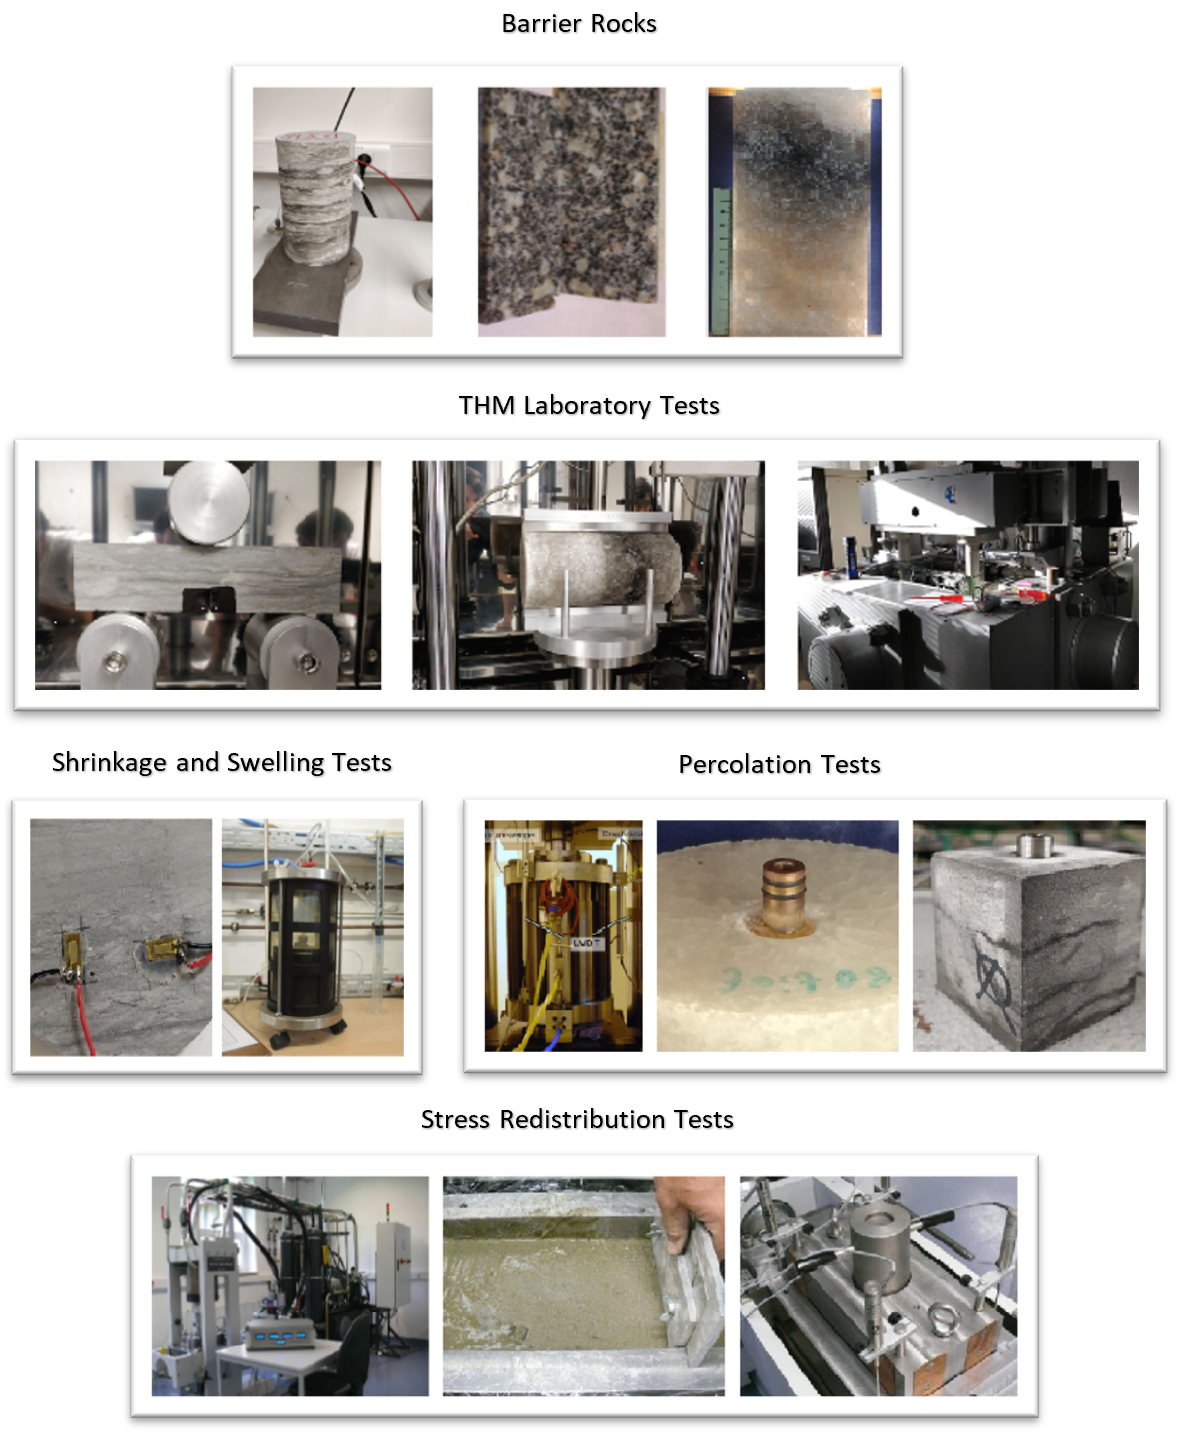
\includegraphics[width=0.95\textwidth]{figures/Amir_Experiment.png}
\caption{The conducted laboratory tests in the scope of GeomInt research project}
\label{fig:Amir_Experiment}
\end{figure} 
%===================================================================================================
\section{Rock Material Properties}
\label{sec:material-properties}
%-----------------------------------------------------------
\subsection{Opalinus Clay from Mont Terri, Switzerland}
\label{subsec:clay}
\Authors{Tilo Kneuker, Bernhard Vowinckel, Markus Furche, Gesa Ziefle, Jobst Ma{\ss}mann}

\subsubsection{The Mont Terri Rock laboratory}\label{sec:mont_terri}
\index{URL Mont Terri}
\index{Opalinus Clay}

Opalinus claystone is a very promising hostrock for the safe disposal of heat emitting nuclear waste. This type of hostrock has been investigated in the Mont Terri Rock laboratory for more than 24 years. The Mont Terri rock laboratory is a facility to conduct research in the deep geological underground at in-situ scale, such as the safe deposition of radioactive waste, where the local host rock is Opalinus Clay. The rock laboratory is located within the Jura Mountain fold belt. The development of the Jura fold belt began in the Middle Miocene around 12 million years ago, which was constrained by the first occurrence of overthrusted and folded molasse sediments \cite{bolliger1993}. The overthrust of the frontal fold and thrust belt over the allochthonous foreland (Tabular Jura) occurred ca. 10.5 million years ago \cite{becker2000}. More specifically, the Mont Terri rock laboratory is located in the southeast dipping fold limb of the NW-vergent Mont Terri anticline \cite{nussbaum2011}. The total amount of shortening of the anticlinal structure is approximately 2.1 km \cite{freivogel2003}. During the folding process, the northwestern fold limb of the Mont Terri anticlinal structure was sheared-off and now lies on top of the Tabular Jura (Figure \ref{fig:bgr_mt_sideview}). The Mont Terri anticlinal structure developed in a special structural setting at the intersection between the frontal part of the Jura fold belt (main shortening direction NW-SE) and the roughly N-S oriented structural elements of the Rhine-Bresse-graben transfer zone \cite{nussbaum2011}.

\begin{figure}[!ht]
\centering
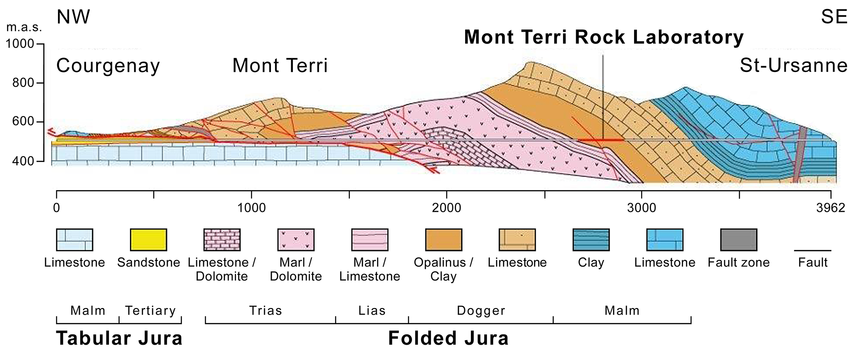
\includegraphics[width=1\textwidth]{./figures/bgr_mont_terri_side_view.png}
\caption{Geological cross section along the motorway tunnel through the Mont Terri anticline. From: Kaufhold et al. (2016) \cite{kaufhold2016}, based on Freivogel \& Huggenberger (2003) \cite{freivogel2003}.}
\label{fig:bgr_mt_sideview}
\end{figure}

The Mont Terri rock laboratory branches off from the security gallery of the motorway tunnel near the town of St. Ursanne (NW Switzerland). The rock laboratory is located mainly within the Middle Jurassic Opalinus Clay formation. The thickness of the Opalinus Clay in the rock laboratory is around 130 m \cite{hostettler2018} and the layers are dipping with ca. 40° towards SE. The depth below ground varies between 230 m and 320 m, depending on the topography \cite{heitzmann2001}. Since 1996, a total of 1400 m of galleries and niches have been excavated in the Mont Terri rock laboratory (Figure \ref{fig:bgr_mt_topview}). The Mont Terri rock laboratory is a generic scientific research laboratory. At Mont Terri, there will be no storage of radioactive waste.

\begin{figure}[!ht]
\centering
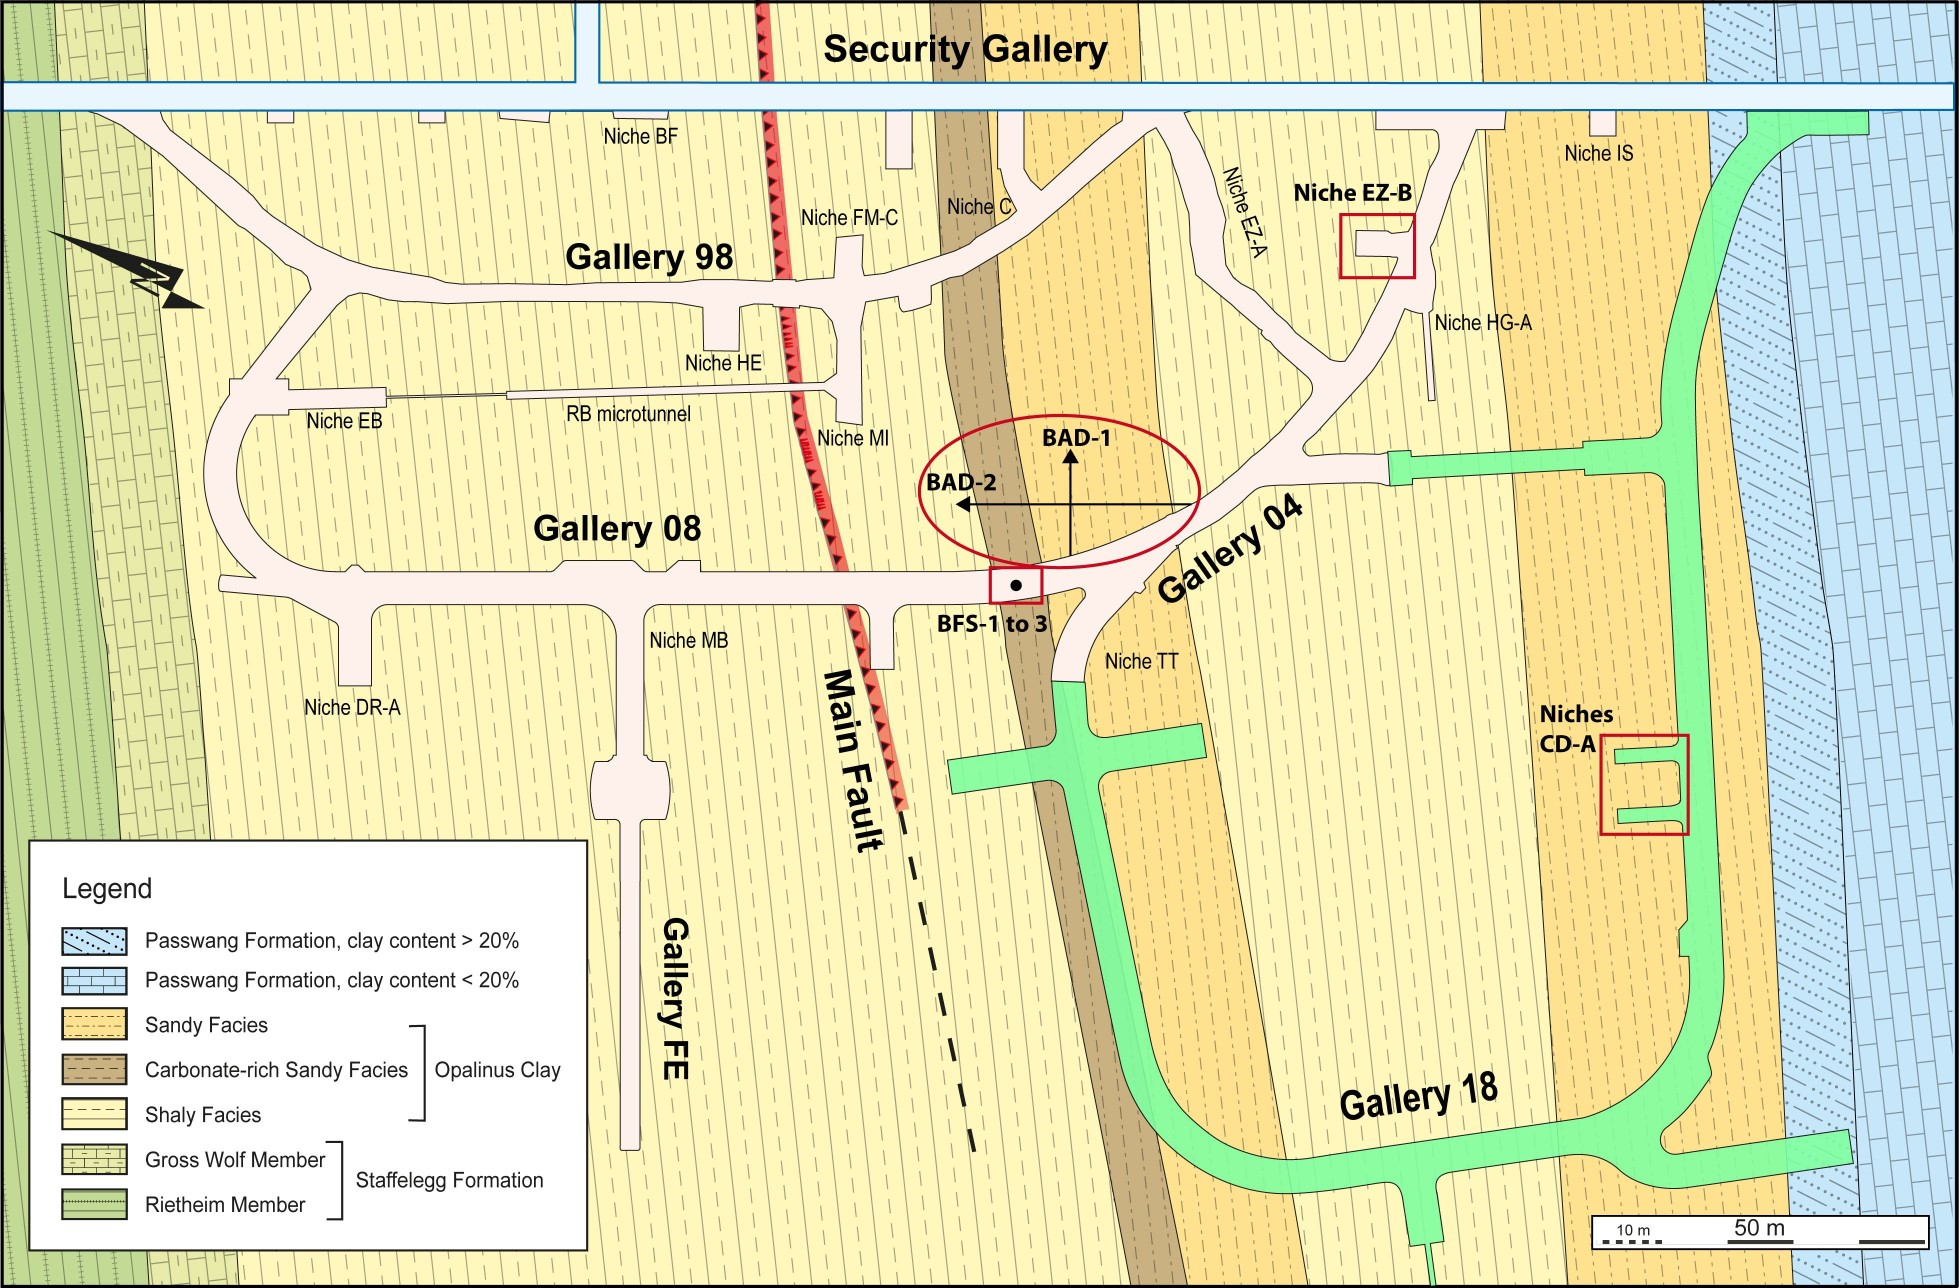
\includegraphics[width=1\textwidth]{./figures/bgr_mont_terri_top_view.jpg}
\caption{Geological map of the rock laboratory with all in-situ experiments relevant for the GeomInt project including the locations of the two AD-boreholes (BAD-1, BAD-2), the drilling for the FS experiment (BFS-1 to 3), the EZ-B niche for the CD/LP experiment and its successor experiment CD-A in Gallery 18. The different facies types of the Opalinus Clay can be recognized by the different shades of brown and yellow, the new Gallery 18 and the new experiment niches are highlighted in green on the map.  (map modified from Mont Terri Consortium, swisstopo).}
\label{fig:bgr_mt_topview}
\end{figure}
\index{MT-CD/LP experiment}
\index{MT-FS experiment}

The Opalinus Clay in the rock laboratory is composed of a dark gray claystone that was named after the ammonite species Leioceras opalinum. This claystone formation was deposited during the period of the Toarcian/Aalenian, at an age of approximately 174 million years. The Opalinus Clay is exposed along the rim of the Swabian and Franconian Alp in Germany and stretches into northern Switzerland \cite{einsele1983}. The Opalinus Clay was deposited in a shallow-marine, epicontinental milieu in the area of the storm wave base at approximately 20 m to 50 m water depth \cite{wetzel2003}. Coarser siliciclastic components are of detritical origin. Potential sources for the detritic components are the areas of the Bohemian Massif and the Vindelician Landmass \cite{wetzel2003}. During Cretaceous burial, the Opalinus Clay experienced maximum palaeo temperatures of $75^{\circ}$~C to $90^{\circ}$~C \cite{bossart2008} at a maximum burial depth of 1.35 km. The Opalinus Clay at the Mont Terri site is underlain by  marls of Upper Toarcian age and overlain by limestones (Bajocian), some of which act as karst aquifer \cite{pearson2003}.
\index{karst aquifer}

The Opalinus Clay at the Mont Terri rock laboratory can be subdivided into three main facies types \cite{bossart2008}. First, the lower shaly facies occupies the largest area of the rock laboratory (Figure \ref{fig:bgr_mt_topview}). It dominates the lower part of the Opalinus Clay formation. It consists of mica-bearing clay and marly shales as well as flasery, marly layers characterized by bioturbation. The upper shaly facies contains a higher volumetric content of quartz grains. Second, the sandy facies occurs in the middle and upper part of the profile (lower and upper sandy facies). It includes medium gray marly claystones with intercalated, bioturbated marly layers or lenticular, gray sandy limestones and pale sand layers of approximately 1-10 mm thickness that include pyrite as well. Third, a carbonate-rich sandy facies of approx. 5 m thickness occurs in the middle part of the rock formation. It consists of calcareous sandstones with intercalated bioturbated limestone layers, which show a relatively high proportion of detritic quartz and white mica. The different facies types of the Opalinus Clay can be attributed to varying sedimentation conditions in a shallow marine environment (like variations in depth and current directions). The carbonate-rich facies is typical for the Jura region in western Switzerland and it does not occur in the proposed siting regions for a deep geological repository in Northern Switzerland.
\index{bioturbation}

The mineralogical composition of the Opalinus Clay was examined by Traber \& Blaser (2013) \cite{traber2013} for several locations in Northern Switzerland. For the shaly facies, the clay mineral content varies between 40 wt\% and 75 wt\%. The clay minerals determined include illite, kaolinite and smectite-illite mixed layer minerals, the proportion of swellable clay minerals is around 10 wt\%. Detritic components such as quartz and feldspars typically make up to 20 wt\% of the investigated samples. The carbonate content (calcite and dolomite) is around 20 wt\%. The sandy facies of the Opalinus Clay is composed of up to 40 wt\% clay minerals and ca. 30 wt\% quartz; it shows a lower amount of clay minerals in favor of a higher quartz content, compared to the shaly facies \cite{heitzmann2001}. 
\index{Opalinus Clay}

The BGR has been involved in a number of campaigns to study in-situ conditions of clay rock, of which the following four are particularly noteworthy within the context of the GeomInt-Project. First, in the CD experiment the long-term cyclic deformation (CD) due to seasonally induced cyclic swelling and shrinkage is investigated in a niche of the rock laboratory. These measurements are continued in the LP (long-term monitoring of pore parameters) experiment. In addition, a follow-up project, the CD-A experiment, has been prepared in recent years, to distinguish between deformation processes due to stress redistribution and seasonal variations in air humidity that cause saturation (swelling) and desaturation (shrinkage) of the rock and stress redistribution alone. To this end, two identical niches were excavated, one sealed towards the gallery and with a high humidity inside to minimize desaturation and one open to the general air circulation of the rock laboratory. The measurement campaign was started in October 2019 \cite{ziefle2019}. Third, the AD experiment (experimental-numerical Analysis of Discontinuities) intends to provide an improved process understanding for the experimental-numerical analysis of discontinuities. Finally, the Fault Slip (FS) – experiment addresses the fault reactivation due to pressure-induced percolation in a low-permeability, large-scale discontinuity in the Mont Terri rock laboratory. The AD is directly relevant to the numerical and experimental investigations presented in Sections \ref{sec:mex05} - \ref{sec:mex12}, because the rock material used in these experiments were drilling samples from the AD experiment. Hence, we provide a brief overview for the campaign in the following. 



\subsubsection{The CD/LP Experiment in the Mont Terri Rock laboratory}
\index{MT-CD/LP experiment}

The Mont Terri Rock laboratory in Switzerland hosts a multitude of in-situ experiments that investigate the response of Opalinus Clay to various geotechnical applications. An overview of the rock laboratory is given in Section \ref{sec:mont_terri}. In particular, the CD (Cyclic Deformation) experiment has been a valuable site to gather experimental data at the in-situ scale to investigate the hydraulic-mechanial coupling induced by swelling and shrinking of Opalinus Clay due to cyclic variations of air humidity. Section \ref{sec:mex10} focuses on the numerical investigation of these processes. Here, we provide a brief overview of the experimental CD campaign at the Mont Terri Rock Laboratory. 

The experiment itself is located in the EZ-B niche (Figure \ref{fig:bgr_mt_topview}). The experiment has been conducted for more than 13 years to provide information on the swelling and shrinkage behavior of Opalinus Clay in the Mont Terri rock laboratory. The idea was to analyze a niche that is not covered by shotcrete. Instead, the clay rock remains in direct contact with the atmospheric conditions of the main gallery for the entire time. Consequently, the swelling and shrinkage is induced by changes in temperature and relative humidity, which can decrease to values as low as 65\% in the winter and reaches values of up to 100\% in the summer. 

\begin{figure}[!ht]
\centering
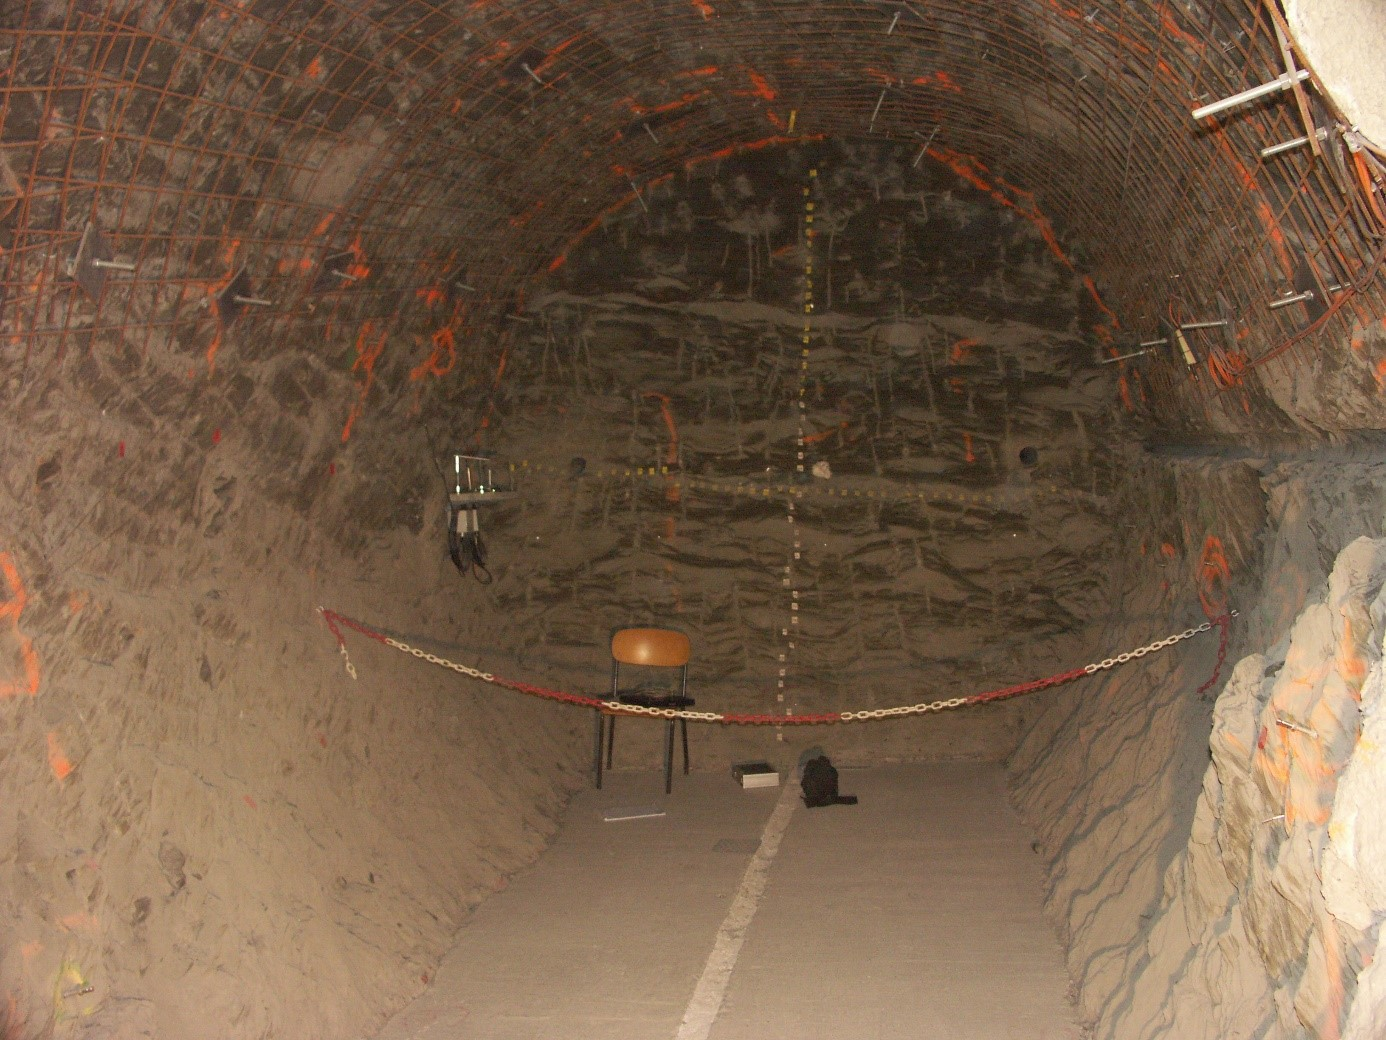
\includegraphics[width=1\textwidth]{./figures/bgr_CD_experiment.jpg}
\caption{The EZ-B niche in the Mont Terri rock laboratory, where the CD/LP experiment has been conducted since 2006 (photo: Mont Terri consortium, swisstopo).}
\label{fig:bgr_CD_experiment}
\end{figure}

A special focus of this experiment was to investigate the long-term impact of these seasonal variations on the temporal evolution of the cracks that occur during the excavation process and make up the Excavation Damaged Zone (EDZ). To this end, the EZ-B niche was excavated in the years 2004/2005 (Figure \ref{fig:bgr_CD_experiment}). Subsequently, the niche was equipped with a comprehensive set of measurement devices to record the evolution of temperature, water content, convergence of the niche and crack development at the tunnel walls over time. This measurement campaign was started in 2006 and has been continued until today to investigate long-term effects. Note that the experiment was transferred into the LP-A experiment to explicitly focus on the long-term monitoring of pore pressure. The CD/LP experiment under in-situ conditions was supplemented by laboratory experiments with drill cores to determine hydraulic-mechanical properties of the clay rock, such as porosity, grain density, etc. \cite{matray2013}. 

Characteristic macroscopic cracks on the tunnel walls have been monitored and the field data of the crack opening show a good correlation with the seasonal variation of temperature and humidity. The cyclic deformation of the crack opening yields a re-occurring compression perpendicular to the crack during summer, which typically is a time of high relative humidity and, hence, the swelling causes an increase of rock volume \cite{jaeggi2012}. This characteristic behavior of swelling and shrinking was successfully reproduced by means of hydraulic-mechanically coupled numerical simulations \cite{ziefle2018}, which provides valuable benchmark data for future investigations of the cyclic deformation of clay rock.

\subsubsection{The AD Experiment}
\index{MT-AD experiment}

The aim of the experiment is to provide core samples from the sandy facies of the Opalinus Clay as a typical example of an argillaceous host rock for the safe disposal of nuclear waste. These samples were used for experimental-numerical analysis in the framework of the GeomInt project. Additionally, a geological characterization of the cores and seismic (Interval Velocity Measurements - IVM) and geolelectrical measurements (Electrical Resistivity Tomography - ERT) in the boreholes were performed. The results of the experimental campaign yield a valuable description of the sandy facies in addition to the well characterized shaly facies of the Opalinus Clay \cite{bossart2008,jahn2016}. 
\index{ERT Electrical Resistivity Tomography}

From a geological perspective, the AD experiment gave opportunity to study the lower sandy facies of the Opalinus Clay at the Mont Terri rock laboratory in detail. The two fully cored boreholes BAD-1 and BAD-2 with a diameter of 131 mm (yielding samples of 101 mm diameter) were drilled parallel and perpendicular to the sedimentary bedding, respectively. The 15.35 m long horizontal borehole BAD-1 was drilled from 7th-10th of July 2018 by the BGR. It is located entirely in the lower sandy facies. The geological mapping was performed by swisstopo \cite{galletti2019}. The core material of BAD-1 was entirely sampled for laboratory experiments performed by the Christian-Albrechts University of Kiel (Germany) and the Institute of Geomechanics (IfG) Leipzig (Germany). The core samples were conditioned in aluminum foil and pressurized in special nitrogen-filled BGR-liners (autoclaves) to avoid further alteration. 

The BAD-2 borehole has a length of 27.0 m. It was drilled by the BGR team from 9th-17th of May 2018. The borehole is oriented perpendicular to the bedding (with a dip of 43°), thus crossing several facies types of the Opalinus Clay. The geological mapping by Swisstopo reported by Galletti \& Jaeggi (2019) \cite{galletti2019} revealed the following sequence with varying quantities of quartz, carbonates (cements and fossils) and clay minerals: 

\begin{list}{-}{\leftmargin=1em \itemindent=0em \itemsep=0em}
\item 0.0 m to 4.75 m depth: upper shaly facies,
\item 4.75 m to 19.4 m depth: lower sandy facies,
\item 19.4 m to 24.57 m depth: carbonate-rich sandy-facies, 
\item 24.57 m to 27.0 m depth: lower shaly facies.
\end{list}

This subdivision is confirmed by petrographic-structural studies and geoelectrical resistivity measurements (ERT) performed by the BGR. The BAD-2 drillcores were sampled from 4.0 m to 14.8 m (lower sandy facies) for laboratory experiments by the Universities of Kiel and IFG Leipzig. Following the procedure employed for the BAD-1 drilling, the core material was conditioned in aluminum foil and pressurized in special nitrogen-filled BGR-liners (autoclaves). The drillcore material from the intervals between 0.0 m to 4.0 m and 14.8 m to 27 m, including the transition towards the underlying carbonate-rich facies, are stored at the BGR facility in Hannover (Germany) for further geological characterization. The first results revealed a good core quality and confirm a rather uniform appearance of the sampled profile inside the lower sandy facies, the drillcore material is thus suitable for the planned experiments (cf. Figure \ref{fig:bgr_AD_experiment}).

\begin{figure}[!ht]
\centering
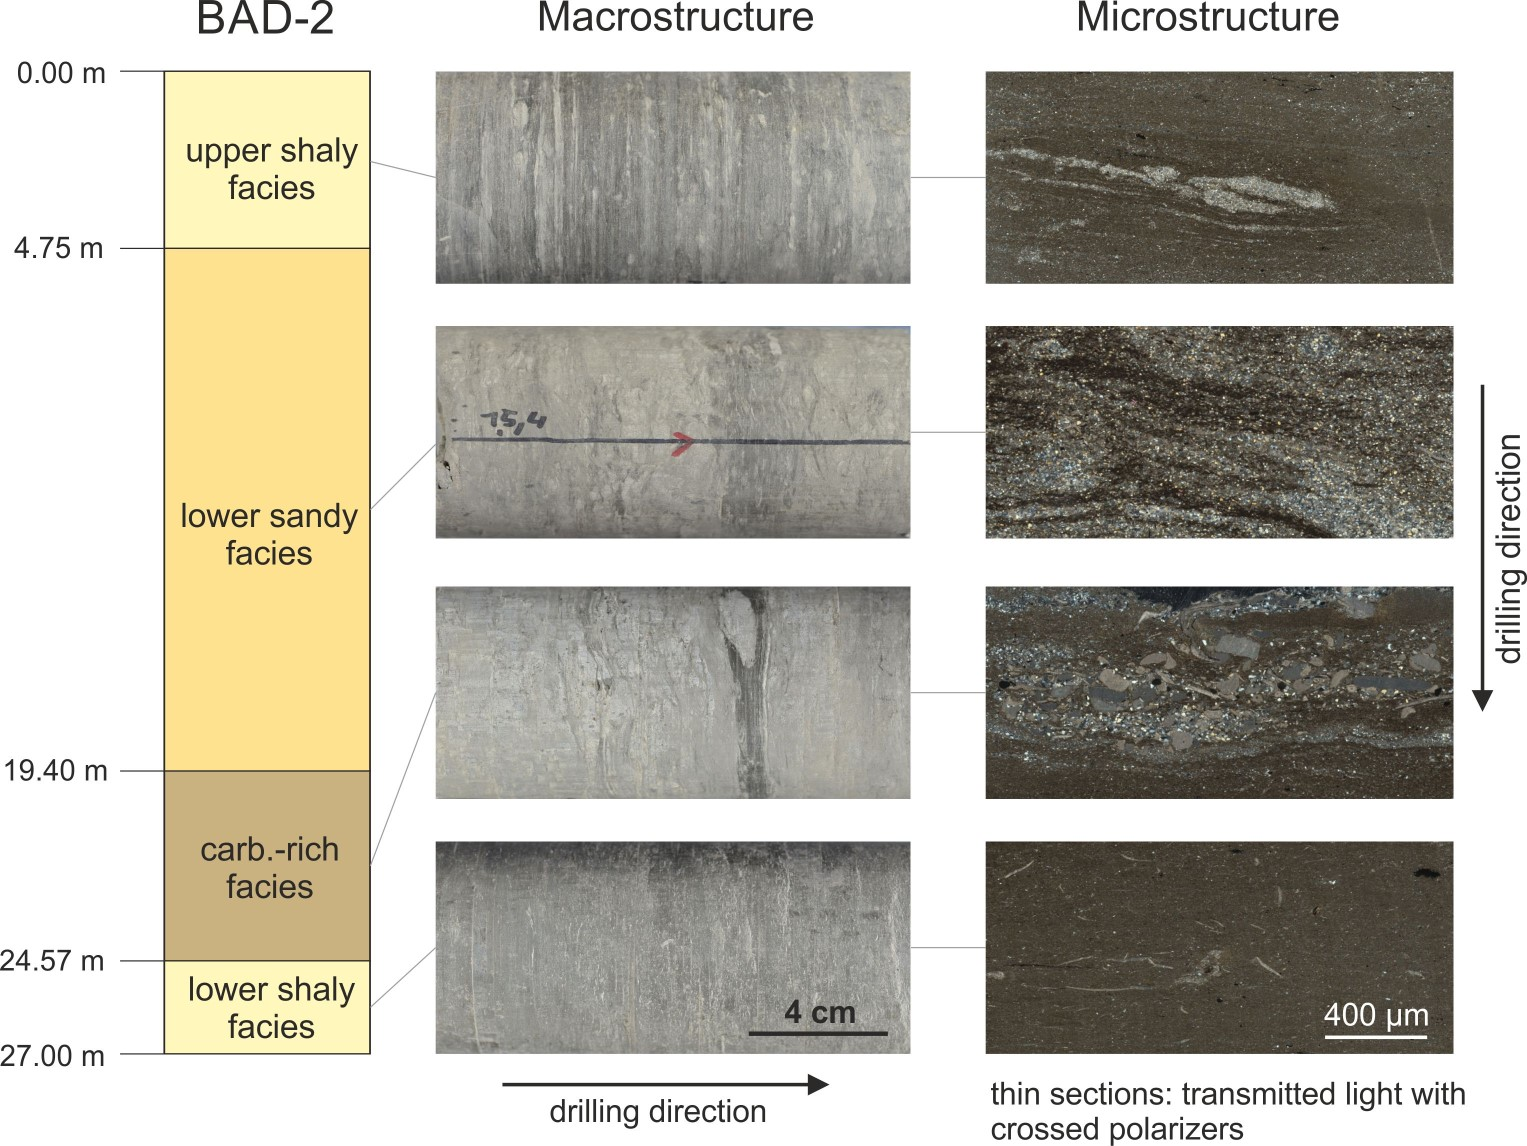
\includegraphics[width=1\textwidth]{./figures/bgr_AD_experiment.jpg}
\caption{Schematic profile of borehole BAD-2 as marked in Figure \ref{fig:bgr_mt_topview} (left), macrostructural (on drillcore scale) and microstructural features (on thin section scale) of the different facies types of Opalinus Clay encountered in the BAD-2 borehole.}
\label{fig:bgr_AD_experiment}
\end{figure}

\textbf{High resolution ERT measurements in borehole BAD-2[Markus Furche]}
\index{ERT Electrical Resistivity Tomography}
The task of geophysics was to characterise the rock unit that had been drilled through, to precisely determine the locations of the facies boundaries and to describe the variability, especially of the sandy facies. The electrical resistivity tomography (ERT) method was used for this purpose.

\textbf{Principle}
To determine the spatial electrical resistivity distribution (or its reciprocal $-$ the electrical conductivity) in the ground, a direct current (DC) is injected into the ground through two point electrodes (A, B), see Figure \ref{fig:four-electrode-array}.
\begin{figure}[!ht]
	\centering
		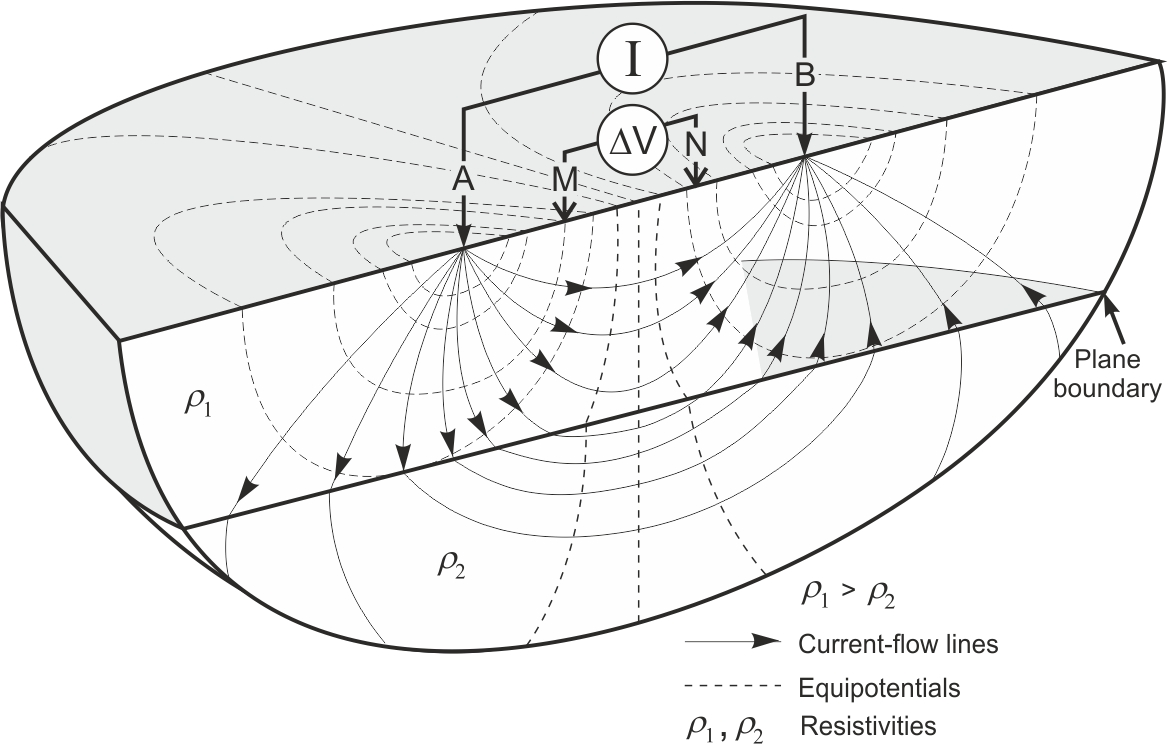
\includegraphics[width=1\textwidth]{./figures/fig-ERT-1.jpg}
	\caption{Principle of resistivity measurement with a four-electrode array (modified after Kn{\"o}del et al., 2007 \cite{knoedel2007}).}
	\label{fig:four-electrode-array}
\end{figure}
The resulting electrical field is measured using two other electrodes (M, N). A point electrode introducing an electrical current $I$ will generate a potential $V_{r}$ at a distance $r$ from the source. In the case of the four-electrode array shown in Figure \ref{fig:four-electrode-array}, the two current electrodes (A, B) introduce a current $I$. When assuming a homogeneous half-space, the potential difference $\Delta V$ between the electrodes M and N can be calculated as:
\begin{equation}
	\Delta V=\rho I \left[\frac{1}{2\pi}\left(\frac{1}{\overline{\rm{AM}}}-\frac{1}{\overline{\rm{AN}}}-\frac{1}{\overline{\rm{BM}}}+\frac{1}{\overline{\rm{BN}}}\right)\right]
\end{equation}
Here, $\overline{\rm{P}_{1}\rm{P}_{2}}$ denotes the distance between two points $\rm{P}_{1}$  and $\rm{P}_{2}$. Replacing the factor in square brackets with $1/K$ , we obtain the resistivity of the homogeneous half space as follows:
\begin{equation}
	\rho=K\frac{\Delta V}{I}.
\end{equation}
The parameter $K$ is called configuration factor or geometric factor. For inhomogeneous conditions, it yields the resistivity of an equivalent homogeneous half-space. For this value the term apparent resistivity $\rho_{a}$ is introduced, which is normally assigned to the center of the electrode array. Multi-electrode resistivity meters enable the measurement of 2D resistivity surveys (2D imaging). The advantages of this kind of measurements are their high vertical and horizontal resolution along the profile. 
An inversion process of the measured data is necessary for the final interpretation. This process transforms the apparent resistivities into a reliable model discretised into a distinct number of elements of homogeneous resistivity. All inversions are performed using the non-commercial software BERT (Boundless Electrical Resistivity Tomography \footnote{https://gitlab.com/resistivity-net/bert}) developed by Th. G{\"u}nther (Leibniz Institute of Applied Geophysics, Hannover) and C. R{\"u}cker (Technical University of Berlin).

\textbf{Measurements and Results}

\begin{figure}[!ht]
	\centering
		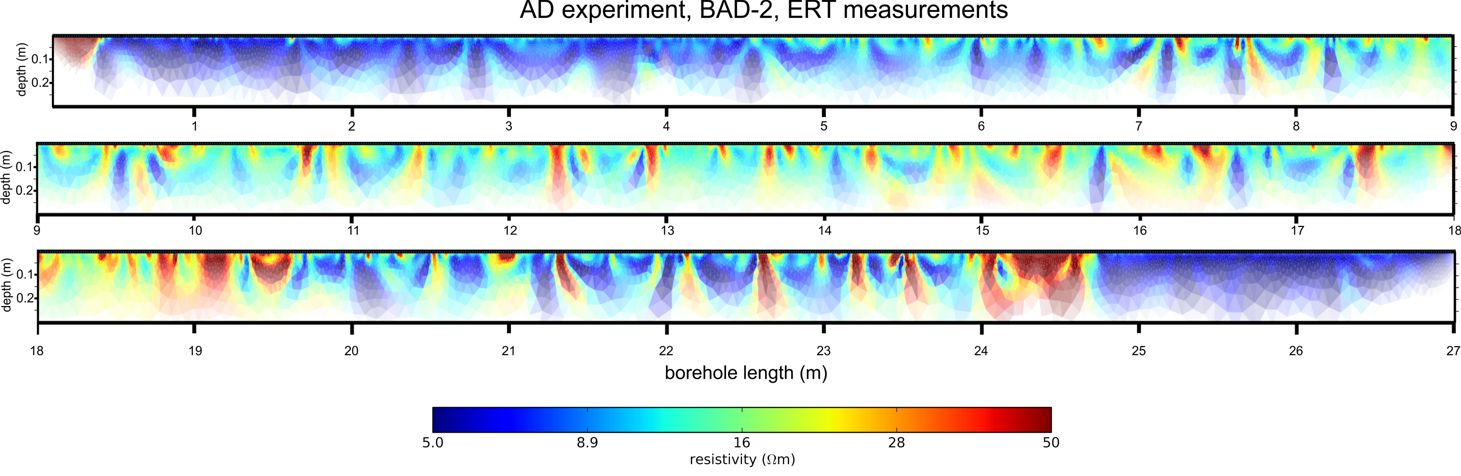
\includegraphics[width=1.35\textwidth, angle=90]{./figures/fig-ERT-2.jpg}
	\caption{Borehole BAD-2: Two-dimensional distribution of the resistivity as a result of the inversion calculation.}
	\label{fig:ERT-2d-model}
\end{figure}
The measurements were performed on May 21$^{\rm{st}}$ and 22$^{\rm{nd}}$ 2019. Since the borehole is perpendicular with respect to the bedding, measurements were only taken in one orientation (0$^{\circ}$, i.e. the electrodes are oriented upwards). Along the borehole, 35 individual profiles of 1.5 m length with half-sided overlapping were measured.

The data processing consists of the following steps: First thing is the scaling of the data in order to eliminate the geometry effects of the borehole. Then data points with high statistic error ($>3 \%$) or high phase angle (absolute value $>$ 100 mrad) were eliminated. 12 or 13 consecutive single data sets were combined to three cumulative ones (00.10 m - 09.85 m, 08.36 m - 18.10 m, 16.61 m - 26.98 m; the last record of the previous section is the first of the following). With these three data sets the inversion was performed using standard parameters. The resulting resistivity models are shown in Figure \ref{fig:ERT-2d-model}.

\begin{figure}[!ht]
	\centering
		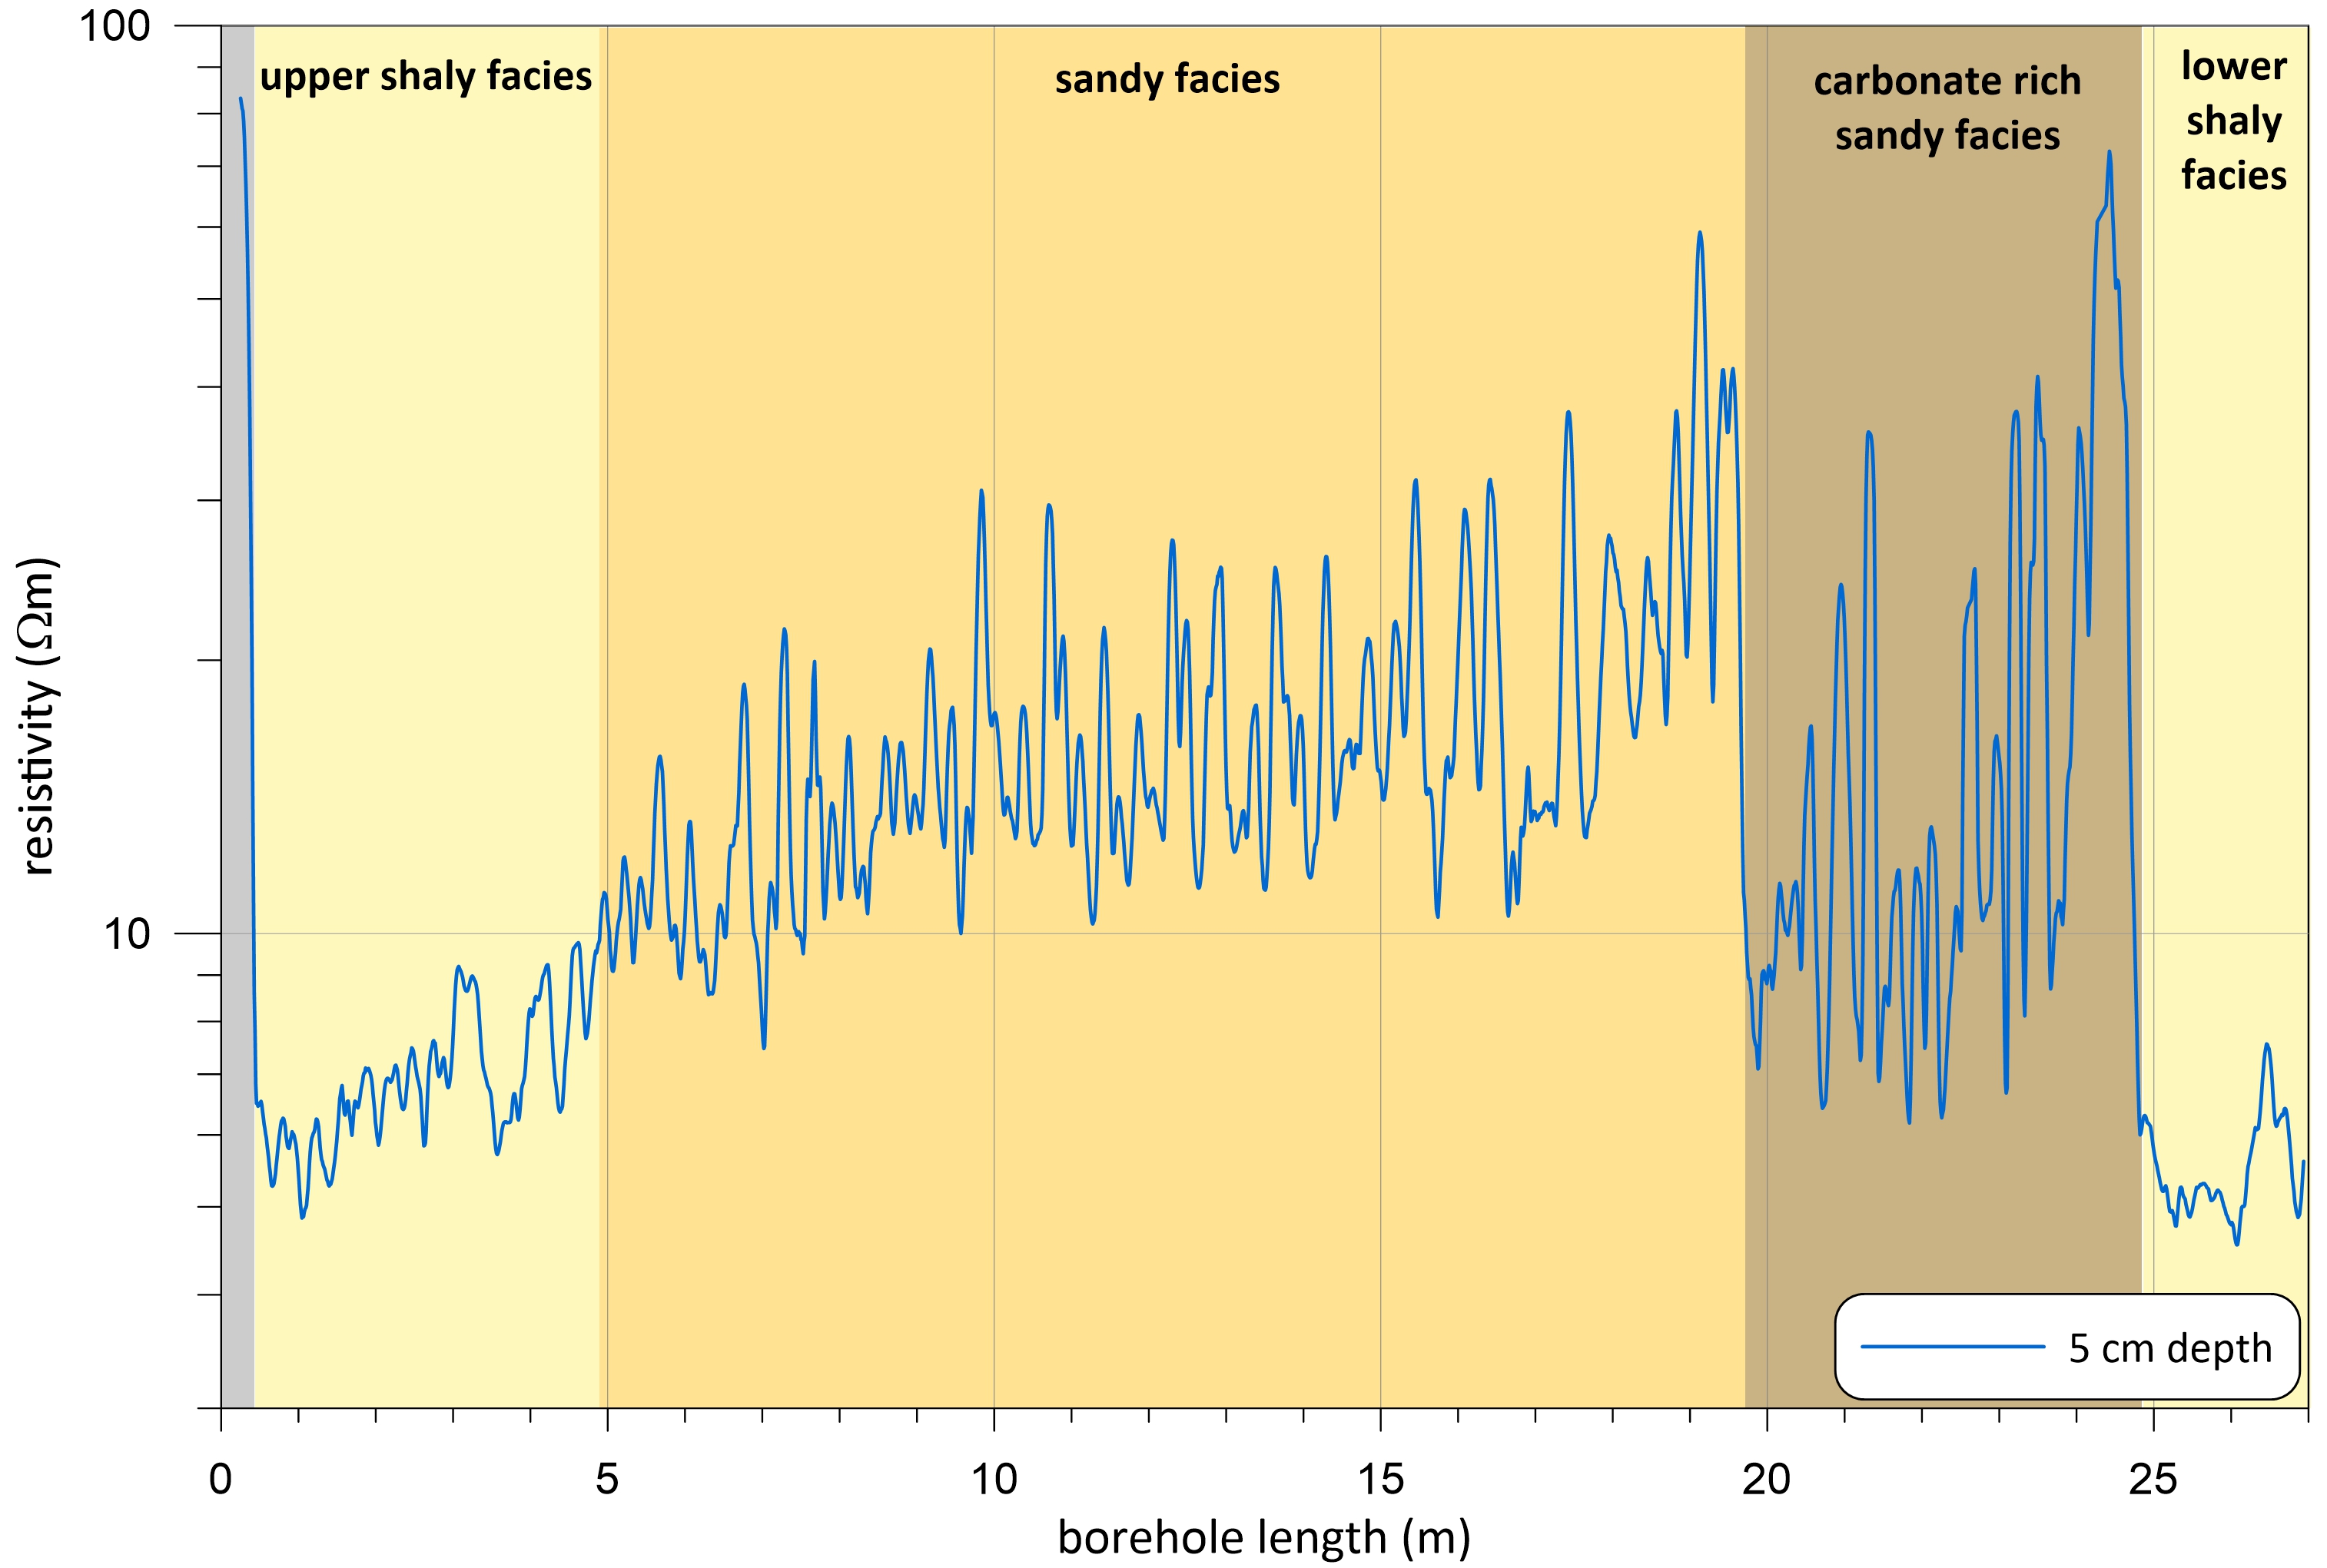
\includegraphics[width=1\textwidth]{./figures/fig-ERT-3.jpg}
	\caption{Borehole BAD-2: Curve of the resistivity at a distance of 5 cm from the borehole wall.}
	\label{fig:ERT-model-curve}
\end{figure}
Up to 50 cm borehole depth, the shotcrete can be recognised as a high-resistance structure. Beyond that, the resistivity is well below 10 $\Omega$m and rises slowly with increasing borehole depth. Embedded in this basic structure are thin layers with high resistivity ($>$ 30 $\Omega$m). Between 18.5 m and 19.5 m, there is a very extensive high-resistance range, after which the resistance level drops significantly, again with embedded high-resistance layers. Between 24.0 m and 24.7 m a second distinct high-resistance range is reached, beyond which a sharp drop to values below 10 $\Omega$m can be observed. This level is maintained down to the bottom of the borehole without further intermediate structures.

From the calculated 2D models of the resistivity, curves can be extracted for specific distances from the borehole wall. Figure \ref{fig:ERT-model-curve} shows the corresponding resistivity curve for a distance of 5 cm. The different facies types are indicated as colour background. It can be seen that both the upper and lower shaly facies are characterised by resistivities below 10 $\Omega$m with little variation. The mean level in the sandy facies (4.9 m to 19.7 m) is significantly higher (about 15 $\Omega$m), and the variability is also considerably greater. Both, the upper and the lower transition towards the carbonate-rich sandy facies are clearly indicated as a sharp drop in the resistance curve. Here, the average level of resistivity lies between the values for shaly and sandy facies, the amplitudes of the variations are highest.

\textbf{Implications of the geological-geophysical investigations}

Petrographic-structural studies form the basis for rock characterization and provide first indications for the compositional-structural variability, which independently is confirmed by geophysical borehole measurements.

ERT is able to characterise structures close to the borehole and to resolve rock variability with high accuracy. The individual facies types of Opalinus Clay can be distinguished based on mean resistivities and the type of heterogeneity (amplitudes and sequence). Especially the important transitions towards the carbonate-rich sandy facies can be precisely located.

The results confirm that the upper shaly facies is closely related to the most homogenous facies type of Opalinus Clay (the lower shaly facies). In contrast, the lower sandy facies and especially the carbonate-rich sandy facies represent the more heterogeneous endmembers of the investigated claystone formation.
The new results are consistent with published data and support the classification of the Opalinus Clay at the Mont Terri site into several major facies types. Further investigations will focus on the characterization of intra-facies variability using the sub-facies concept.




\clearpage
%---------------------------------------------------------------------------------------------------
\subsection{Rock Salt Samples}
\label{subsec:salt}
\Authors{Mathias Nest, Dirk Naumann (IfG)}

\subsubsection{The Springen in-situ laboratory}
\label{sec:springen}

The large-scale test site Merkers benefits from the unique mining situation in the bedded salt mass of the Werra salt formation (z1, Zechstein sequence) where two potash seams were mined in a room-and-pillar system at 275 m (1st floor, potash seam ''Hessen'', z1KH) and 360 m (2nd floor, potash seam ''Thüringen'', z1KTh) depth, respectively. Fig. \ref{fig:springenlab} shows the preparation of an experiment on the 2nd seam. The evaporite rocks of the Zechstein formation were laid down during the Permian period around 250 million years ago. The intact mineral deposit was locally disturbed between 14 and 25 million years ago by tertiary volcanism, leading to the mutation of some potash salts to sylvinite, and the creation of pockets of CO$_2$ under high pressure.

\begin{figure}[ht!]
\centering
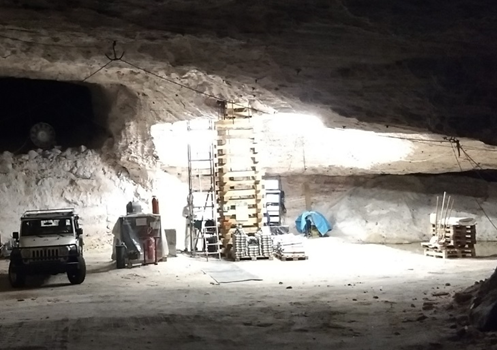
\includegraphics[width=0.85\textwidth]{figures/springen2ndseam.png}
\caption{Preparation of experiments on the second seam.}
\label{fig:springenlab}
\end{figure}

The pressurized tests are conducted between the two potash seams in the very homogeneous Middle Werra rocksalt (z1Na). It consists mostly of very pure halite layers intersected by thin anhydrite lines or bands of rocksalt with finely distributed anhydrite accessories indicating the sedimentary bedding. 

Because the test results depend mainly on the acting stress field, i.e. the minimal stress distribution in the rock mass around the test area, it has been measured and  characterized by hydro-frac measurements, and is thus well-known. The minimal stresses in the contour increase with progressive distances from the underground openings until reaching a constant value in a depth of around 15 m. The measured value of an undisturbed stress state of around 8 MPa corresponds fairly well to calculated lithostatic stresses of 7.8 to 8.8 MPa. 

The main facility is a large borehole of nearly vertical 60 m height and 1.3 m diameter. It was drilled upwards from the second floor, ending about 20 m beneath the first floor. For access to the later sealed volume an 85 mm pilot hole has been drilled from the upper floor. The borehole was closed by a 20 m high MgO-concrete plug. 

For monitoring of micro-seismic events, e.g. due to creation of an excavated damage zone around underground openings or fluid flow driven damage, a highly sensitive AE-network was installed in observation boreholes, which were drilled parallel to the main borehole. This network has constantly been updated and extended over the past years. Signals of magnitude M $<$ -4 can be detected in a frequency range from 1 kHz to 200 kHz. This corresponds to intergranular microcracking on grain boundaries on a millimeter- to centimeter-scale. 

\subsubsection{Rock salt laboratory}

The following conditions and equipment are available in the IfG labs for rock mechanical laboratory investigations:

\begin{list}{-}{\leftmargin=1em \itemindent=0em \itemsep=0.1em}
\item Climate-controlled rooms for storage of specimens at conditions which correspond to those present in situ
\item Laboratory for mineral-petrographic examinations, density and moisture determination, ultra-sound measurements and 
photographic documentation
\item Workshop for the preparation of specimens in high precision according to testing requirements (rock saws, lathes etc.)
\item Test laboratory containing various servo-controlled hydraulic testing machines for conducting investigations on 
rock mechanics in accordance with the up-to-date state of research and development (see Figure \ref{fig:ifglabph1}).
\end{list} 

\begin{figure}[!ht]
\centering
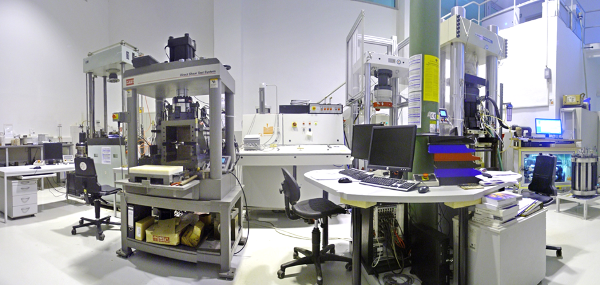
\includegraphics[width=1\textwidth]{./figures/ifg-lab-photo1-v2.png}
\caption{View inside the rock mechanical lab with various servo-controlled hydraulic testing machines.}
\label{fig:ifglabph1}
\end{figure}

It has to be mentioned that some of the applied IfG test procedures have been developed for the requirements of the specific IfG-material laws. 
But generally they are in accordance to ASTM and ISRM standards resp. equivalent descriptions, e.g.:

\begin{list}{-}{\leftmargin=1em \itemindent=0em \itemsep=0.1em}
\item ASTM D 4543-85 Standard Practice for Preparing Rock Core Specimens and Determining Dimensional and Shape Tolerances
\item ASTM D 2845-05 Standard Test Method for Laboratory Determination of Pulse Velocities and Ultrasonic Elastic Constants of Rock
\item ASTM D 2664-86 Standard Test for Triaxial Compressive Strength of Un\-drained Rock Core Specimens without Pore Pressure Measurements 
\item DGEG (1979):   Empfehlung Nr. 2 des AK 19 der DGEG (Dreiaxiale Druckversuche).
\item ASTM D4406-04 Standard Test Method for Creep of Cylindrical Rock Core Specimens in Triaxial Compression
\item ASTM D7070-04 Standard Test Method for Creep of Rock Core Under Constant Stress and Temperature
\item ISRM: Suggested Methods for Determining o the Uniaxial Compressive Strength and Deformability of Rock Materials
\item ISRM: Suggested Methods : Part 2 : 2007 - Unconfined Compressive Strength with Young's Modulus and Poisson's Ratio
\item ISRM: - Suggested Methods : Part 2 : Received 1983 - Strength of Rock Material in Triaxial Compression
\end{list}

\subsubsection{Sample characterization and pre-investigation}

Several preliminary investigations are usually done before lab testing. After preparing the cylindric samples (cutting with a rock saw and smoothing the samples with a lathe) in the IfG labs, their density is determined by measuring the geometrical dimensions and the mass. Concerning the quality of these parameters an accuracy in length determination is $<$ 0.01 mm, those in mass determination is $<$ 0.01 g. 

Additionally, ultrasonic investigations are carried out to check integrity, homogeneity and isotropy of the samples. The ultrasonic pulse measurement system used for transmission of the rock specimens consists of two transducer sets for P-waves and S-waves and a receiver system for generating and evaluating the ultrasonic signals. The specimen is placed in physical contact between two piezoelectric transducers, one acts as a driver and the other one acts as a receiver. The transit time of the mechanical pulse to pass through the specimen is used to determine elastic wave velocity.

For samples where both P- and S-waves were measured in axial sample direction the elastic constants are obtained from density ($\rho$) and the ultrasonic velocities ($v_p$, $v_s$) using the following expressions derived from the theory of elasticity for homogeneous, isotropic solids:

\begin{equation}
\label{eq:YoungsModulus_Ultrasonic}
E_{dyn} = \frac{\rho v_s^2(3v_p^2-4v_s^2)}{v_p^2-v_s^2} 
\end{equation}
\begin{equation}
\label{eq:PoissonsRatio_Ultrasonic}
\nu_{dyn} = \frac{v_p^2-2v_s^2}{2(v_p^2-v_s^2)}
\end{equation}

Dynamic elastic parameters of the various rock portions determined on the base of sonic wave velocity at room temperature are in a wide range representing typical values for the various materials as known from other locations. 


\clearpage
%---------------------------------------------------------------------------------------------------
\subsection{Crystalline Rock Samples}
\label{subsec:crystalline}
\Authors{TU Freiberg}

\subsubsection{URL Reiche Zeche Freiberg}\index{URL Reiche Zeche}

\todod{[TUBAF](): Noch eine Abbildung zur Reiche Zeche?}

\begin{wrapfigure}{l}{6cm}
\centering
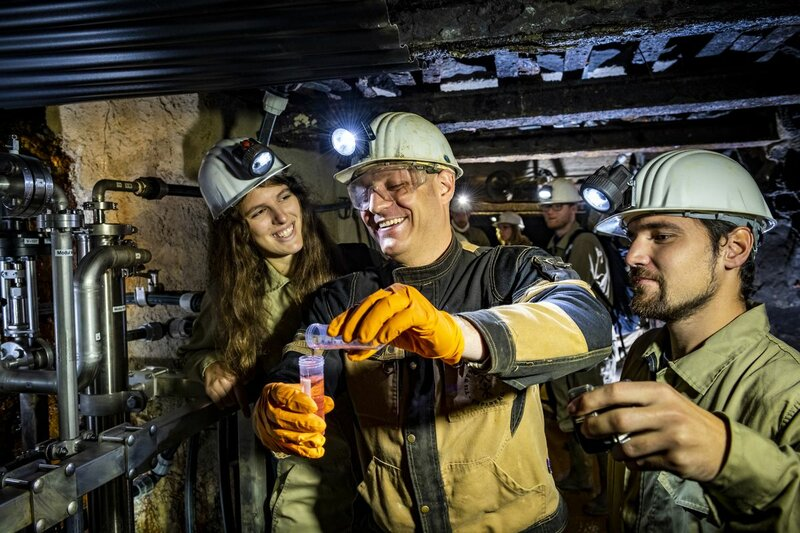
\includegraphics[width=5.9cm]{figures/reiche-zeche.jpg}
\caption{The Reiche Zeche in Freiberg, \cite{ReicheZechePicture}.}
\end{wrapfigure}
The Reiche Zeche mine is located north-east the city center of Freiberg, Saxony. It operated as a silver mine for several centuries. It became a part of the TU Freiberg 1919 when silver mining definitely was no longer profitable. Nowadays the mine is used as an underground research laboratory (URL) and for teaching purposes. The roughly $4\,\text{km}^2$ sized area is well documented in terms of geology, mineralogy, geophysics and geometry. Draining of the mine is done using the "Rothsch\"onberger Stollen (tunnel)". A detailed overview about the history of the Reiche Zeche can be found in \cite{ReicheZecheHistory}.

Due to its long history, the development of new technologies and the importance for the development of the whole region the mining sites and the associated infrastructure are listed as UNESCO world heritage site since 2019.

Current projects are for example dealing with bio-leaching or complex experiments which study the influence of hydro-fracking experiments on the stress state (STIMTEC project).

The Reiche Zeche is equipped with an underground railway system, installed electricity, water and air pressure. The experienced staff and the nearby located mining agency help to successfully conduct experiments in about 150 m depth. 

\clearpage
\subsubsection{Rock material used in the direct shear tests}

\begin{figure}
\begin{subfigure}[c]{0.5\textwidth}
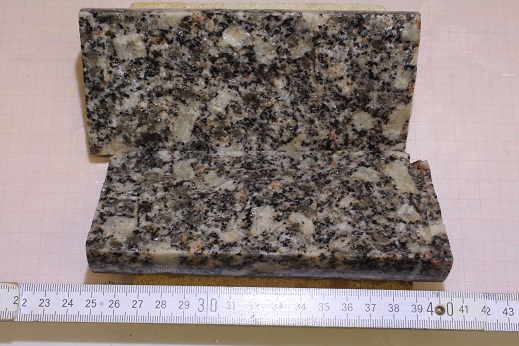
\includegraphics[width=0.99\textwidth]{./figures/ExpRockGranite.JPG}
\subcaption{Granite sample}
\label{fig:RockGranite}
\end{subfigure}
\begin{subfigure}[c]{0.5\textwidth}
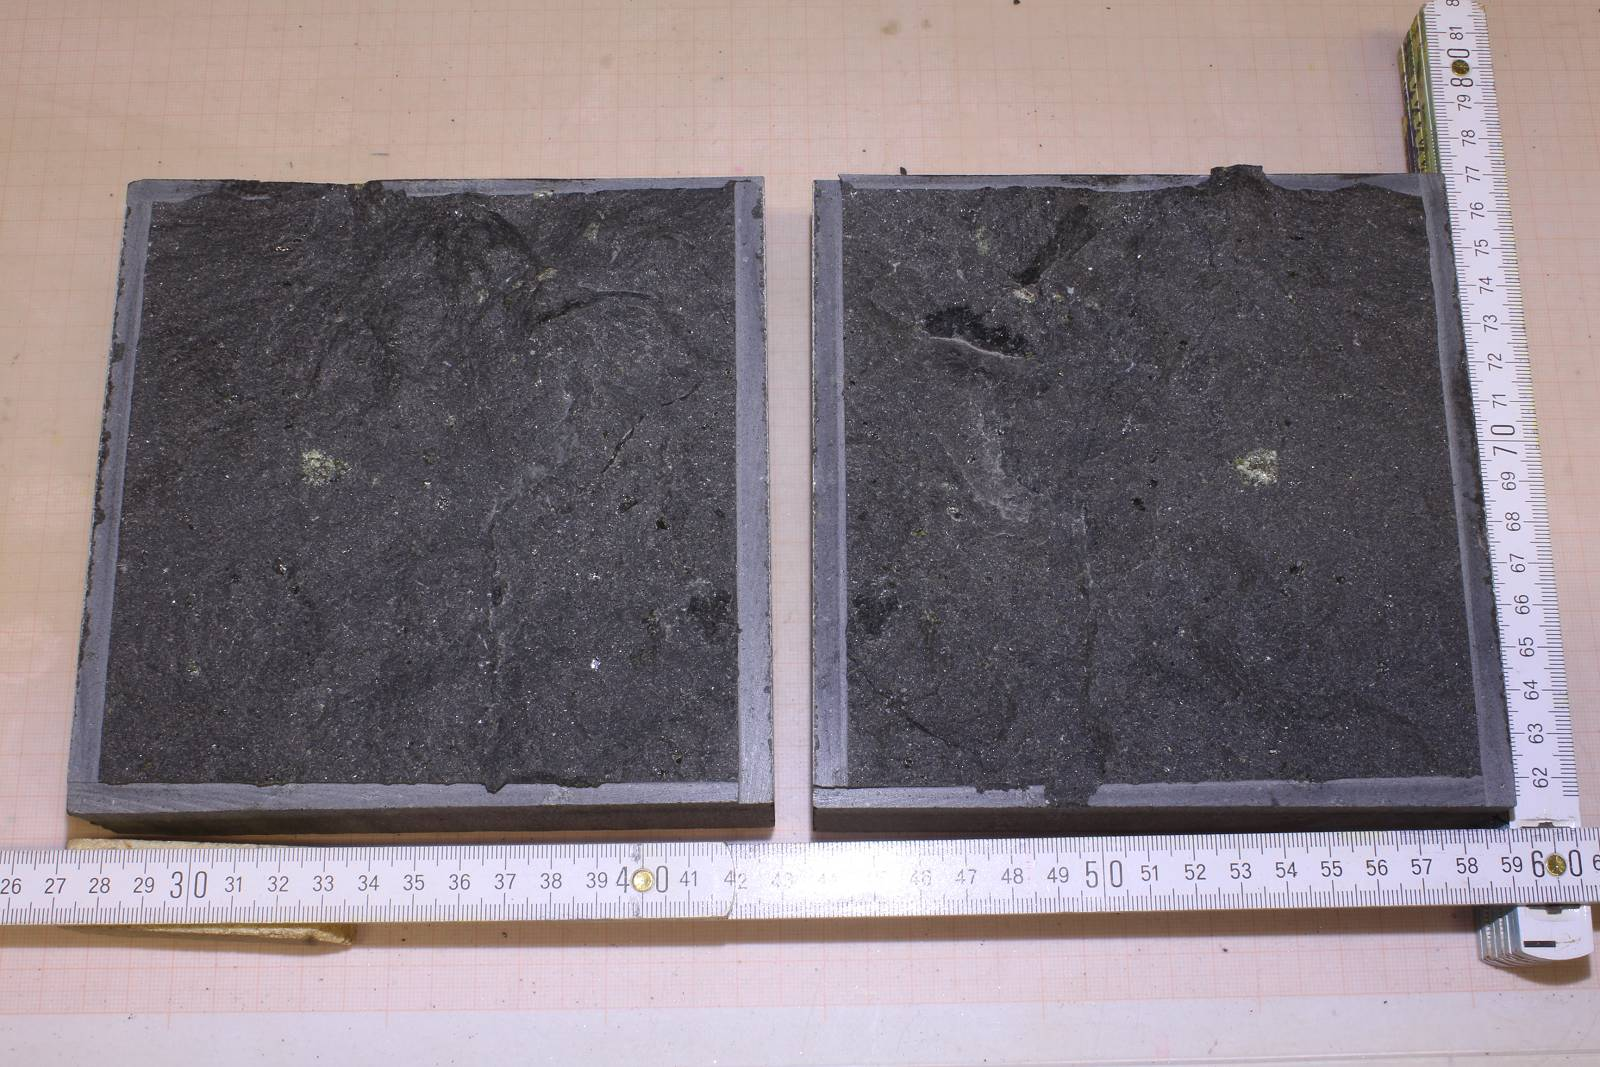
\includegraphics[width=0.99\textwidth]{./figures/ExpRockBasalt.jpg}
\subcaption{Basalt sample}
\label{fig:RockBasalt}
\end{subfigure}
\caption{Crystalline rock samples under investigation}
\end{figure}

Two different crystalline rock \index{crystalline rock} types are used. Granite is a coarse-grained intrusive igneous rock. The grains are on the millimetre to centimetre scale, see Fig. \ref{fig:RockGranite}. The typical main minerals of granites are quartz, feldspar and plagioclase. The used granite origins from Kirchberg, Saxony.
%
Basalt is an fine-grained extrusive igneous rock. It is rich of plagioclase. See Fig. \ref{fig:RockBasalt}. Its origin is V\"olkershausen, Thuringia.
%
Lab tests to evaluate basic rock parameters of the intact rock material have been conducted. The values of the granite and basalt used in the experiments can be found in Tab. \ref{table:MEX7_rockParam}.

\begin{table}[!ht]
\begin{center}
\begin{tabular}{l c r r r}
variable & symbol & granite & basalt & unit\\
\hline
density & $\rho$ & $2.59$ &3.06 &$\text{g}/\text{cm}^3$\\
compressive strength & $\sigma_c$ & $120.54$&272.92 &$\text{MPa}   $\\
tensile strength & $\sigma_t$ & $7.02$&16.61 &$ \text{MPa}   $\\
%static elastic modulus & $E_s$ & $50.00$& &$ \text{GPa}   $\\
elastic modulus & $E$ & $49.75$&105.46 &$ \text{GPa}   $\\
Poisson's ratio & $\nu$ & 0.26 & 0.26  & -\\
fracture toughness & $K_I$ & $0.95$& 2.61 &$\text{MPa}\cdot\text{m}^{0.5}$\\
friction angle (Mohr) & $\Phi$ &  $52.5$& 44 &$^\circ$\\
cohesion & $c$ &  $22.5$& 25.00  &$ \text{MPa}   $\\
basic friction angle &$\varphi_b$ &30 & 31.2 & $^\circ$\\
\end{tabular}
\caption{Rock parameters of granite and basalt used in the direct shear tests.}
\label{table:MEX7_rockParam}
\end{center}
\end{table}

The elastic modulus and the compressive strength were determined using uni-axial compression tests. For the tensile strength a tension test was conducted and the fracture toughness is evaluated by a bending test. The cohesion was determined through a shear test using a saw-cut joint. Ultrasonic measurements were used to determine the Poisson's ratio.
%
The basic friction angles were determined based on \cite{Alejano20121023}. The inner friction angle of basalt is from \cite{Schultz19951} and of granite from \cite{Lanaro2005} and \cite{Ramana2019273}.

\subsubsection{Rock Surface Scanning}
\todo[inline]{[TUBAF](): What about the rock surface scanning? for section \ref{sec:material-properties} ?}
Important measurements to characterise a rock surface are surface scans. In the laboratory of the TU Freiberg a white light scanner is used, see Fig. \ref{TUBAFScanner}. It is a non-contact method which uses monochromatic light. A fringe projection is done and surface scans of rock samples with a resolution of about $30-50 \unit{\mu m}$ can be calculated. Further details about the scanning device can be found in \cite{TUBAFScanningDevice}. 

\begin{figure}[!ht]
\centering
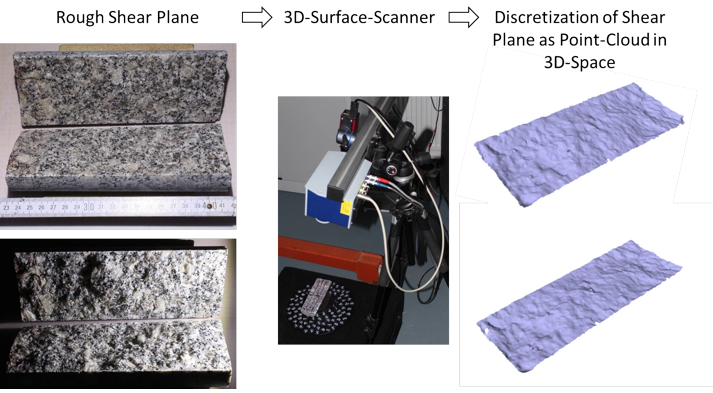
\includegraphics[width=0.95\textwidth]{figures/geomint-wp3-12a}
\caption{Surface scanning. A rock surface is digitized using a surface scanning device. The result is a point cloud.}\label{TUBAFScanner}
\end{figure}
\clearpage
%---------------------------------------------------------------------------------------------------
%===================================================================================================
\section{Thermo-Hydro-Mechanical Laboratory Tests}
\label{sec:thm-lab-tests}
In this section basic methods for rock characterization are briefly introduced such as 
characterization of rock structure (sec. \ref{subsec:structure}),
fracture toughness as materials resistance to fracture propagation (sec. \ref{sec:Fracture_Toughness_Exp}),
Brazilian tests to determine split tensile strength (sec. \ref{sec:Brazilian_Disk_Exp},
and triaxial tests to investigate the three-dimensional strain-strength behavior (sec. \ref{sec:True_Triaxial_Exp}).
%---------------------------------------------------------------------------------------------------
\subsection{X-ray Micro Computed Tomography}
\label{subsec:structure}
\Authors{Matthias Ruf (UoS)}
\index{XRCT X-ray Micro Computed Tomography}

X-ray micro computed tomography ({\textmu}XRCT) is a non-destructive imaging technique and provides the possibility to examine the inner structure of an object by creating a digital 3D image of the same. It is based on the mathematical combination, called reconstruction, of several radiograms which were acquired from different directions. Thereby, a radiogram represents the respective measured intensity values $I(L)$ of the X-rays at position $x = L$ after travelling through the object and can be related to the unattenuated X-rays intensity $I_0$ before the object at position $x = 0$ by the Beer-Lambert law. Under the assumption of a monochromatic X-ray beam this can be written as 

\begin{align*}
I(L) = I_0 \exp\left(-\int_0^L \mu(x) \mathrm{d}x \right)
\end{align*}

for an inhomogeneous material with the unknown material depending attenuation coefficients $\mu(x)$ which are determined during the reconstruction process, cf. \cite{Carmignato2018}.
\index{Beer-Lambert law}

In Figure~\ref{fig:CTsystem} the self-made open and modular {\textmu}XRCT system at the Institute of Applied Mechanics - Chair of Continuum Mechanics of the University of Stuttgart, see \cite{Ruf2020} is depicted. 

\begin{figure*}[ht]
\centering
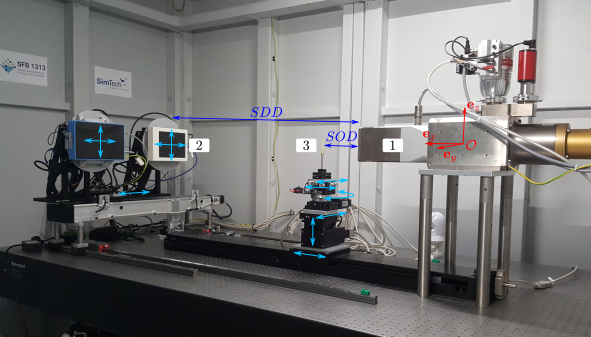
\includegraphics[width=1.0\textwidth]{figures/exp_2_2_xray_main.png}
\caption{Overview of the {\textmu}XRCT-system. The light blue arrows show the possible moving directions of the motorized stages.}
\label{fig:CTsystem}
\end{figure*}

It consists of the three main components: The X-ray source (1), the X-ray detector (2) and the sample positioning system including the rotation stage in between (3). Like most industrial CT-systems the specimen is rotated during the scan and the remaining parts are fixed. The employed X-ray tube provides a maximum power up to \SI{80}{\watt} and at the same time a focal spot size down to \SI{3}{\micro\meter} for moderate power levels. The acceleration voltage of the tube can be adjusted in the range of \SI{30}{\kilo\volt} to \SI{180}{\kilo\volt} and the flux from \SI{10}{\micro\ampere} to \SI{1000}{\micro\ampere}. It can be chosen between two indirect conversion flat panel detectors with different characteristics and resolutions of $1944 \times 1536$ and $2940 \times 2304$ pixels. Both produce gray value images with a pixel depth of \SI{14}{bit} and each is separately mounted on high accurate, motorized XY stages. The latter offers the possibility to compensate for bad detector pixels by taking several images from slightly different detector positions and subsequently stitching of the same to improve the final image quality.

The geometric magnification $M$ is given by the relation of the source detector distance $SDD$ to the source object distance $SOD$, $M = SOD/SDD$, and can be adjusted in a wide range. Depending on the sample material and the smallest feature size of interest, the specimen's diameter can be up to \SI{100}{\milli\meter}. The maximum achievable spatial resolution of the system is about \SI{50}{lp/mm} at \SI{10}{\%} of the modulation transfer function (MTF) which means a smallest feature size of \SI{10}{\micro\meter} that can be resolved. The corresponding field of view for this case is \SI{5.88}{\milli\meter} in width and \SI{4.60}{\milli\meter} in height. Therefore, the smallest expedient sample diameter is about \SI{5}{\milli\meter}. The open and modular concept of the CT-system provides a broad range also for unconventional investigations.

In Figure~\ref{fig:exampleCarraraMarble} a CT scan of a cylindrical Carrara marble core with a diameter of \SI{5}{\milli\meter} for a high resolution scan is shown exemplarily.
\begin{figure*}[ht]
	\centering
    \begin{subfigure}[c]{0.49\textwidth}
    \centering
	\label{fig:exampleCarraraMarble3D}
	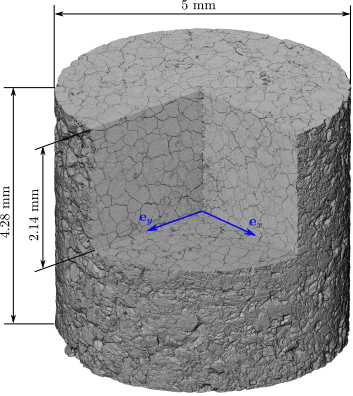
\includegraphics[width=0.9\textwidth]{figures/exp_2_2_scan_3d.png}
    \end{subfigure}
    \begin{subfigure}[c]{0.49\textwidth}
    \label{fig:exampleCarraraMarble2D}
	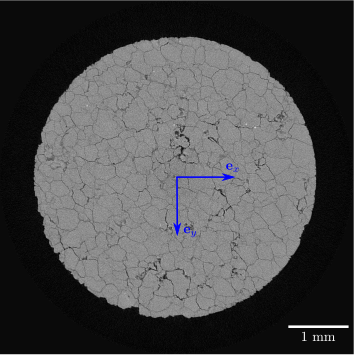
\includegraphics[width=0.9\textwidth]{figures/exp_2_2_scan_2d.png}
\end{subfigure}
\caption{CT scan of a Carrara marble core after thermal treatment.}
\label{fig:exampleCarraraMarble}
\end{figure*}

The visible micro-cracks along the grain boundaries were created by thermal treatment and are not present in the virgin state.  The geometric magnification was set to $M = 24.76$ which corresponds to the highest achievable spatial resolution and leads to a voxel size of \SI{2}{\micro\meter}. For additional details see \cite{Ruf2020}. Besides a qualitative assessment, the data sets offer the possibility of deriving several additional information by image processing. For instance, in geosciences the 3D pore characterization, the 3D grain analysis and the fracture analysis, cf. \cite{Cnudde2013}. 
%---------------------------------------------------------------------------------------------------
%% -----------------Fracture toughness (CAU Kiel)
\subsection{Fracture Toughness of the Opalinus Claystone}
\label{sec:Fracture_Toughness_Exp}
\Authors{CAU Kiel}

In linear elastic fracture mechanics, a materials resistance to fracture propagation is known as fracture toughness. The unit of the fracture toughness is $Pa.\sqrt m$ and the fracture toughness is measured under coupled or individual three different fracture modes I, II and III. In a three-point bending test, the flexural strength ($\sigma_{flex}$), flexural Young's modulus ($E_{flex}$) and flexural strain ($\epsilon_{flex}$) parameters are measured. The fracture toughness test using the three-point bending test provides the Mode I fracture toughness ($K_{Ic}$) of the material (Fig.  \ref{fig:Amir_Fracture_Toughness_Theory}).
\index{fracture toughness}
\index{three-point bending test}

\begin{figure}[!ht]
\centering
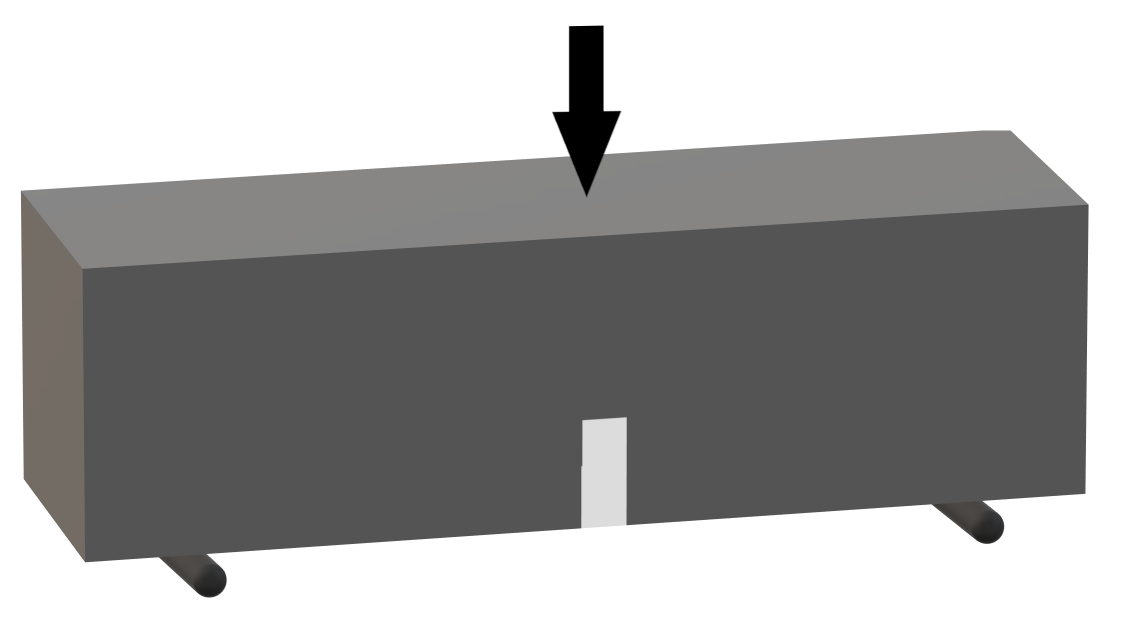
\includegraphics[width=6cm,height=3cm]{figures/Amir_Fracture_Toughness_Theory.png}
\caption{The fracture toughness assessment using three-point bending test}
\label{fig:Amir_Fracture_Toughness_Theory}
\end{figure} 

The stress intensity factor ($K_I$) on the crack tip of predefined notch is obtained with equation (\ref{eq:Fracture_Toughness}) \cite{Bower2009},

\begin{multline}
\label{eq:Fracture_Toughness}
K_I=
\frac{4f_{flex}}{B_{flex}}
\sqrt{\frac{\pi}{W_{flex}}}
\left(1.6
\left(\frac{a_{flex}}{W_{flex}}\right)^\frac{1}{2}
-
2.6\left(\frac{a_{flex}}{W_{flex}}\right)^\frac{3}{2} 
\right.
\\ 
\left.
+12.3\left(\frac{a_{flex}}{W_{flex}}\right)^\frac{5}{2} -21.2\left(\frac{a_{flex}}{W_{flex}}\right)^\frac{7}{2}
+21.8\left(\frac{a_{flex}}{W_{flex}}\right)^\frac{9}{2}
\right)
\end{multline}

where, $f_{flex}$ is the flexural load, $a_{flex}$ is the length of the pre-defined notch, $B_{flex}$ and $W_{flex}$ are the thickness and height of the sample under the flexural test, respectively. During the test procedure, the load and crack mouth opening displacement (CMOD) values are measured and plotted. At the load in which the crack starts to propagate into the medium the fracture toughness $K_{Ic}$ is calculated. In order to perform the fracture toughness test, a loading cell with three rolling supports is required (Fig. \ref{fig:Amir_Fracture_Toughness_Setup_a}). However, the in-situ condition can only be reached when a material is under controlled temperature and humidity conditions. Therefore, a climate chamber in a laboratory of CAU Kiel has been utilized to reach the desired temperature and humidity (Fig. \ref{fig:Amir_Fracture_Toughness_Setup_b}). The temperature can be controlled between 20 to 80 $^{\circ}C$ and relative humidity varies from 0 up to 100. 
\index{crack mouth opening displacement (CMOD)}

\begin{figure}[!ht]
\centering
\begin{subfigure}[c]{0.6\textwidth}
\centering
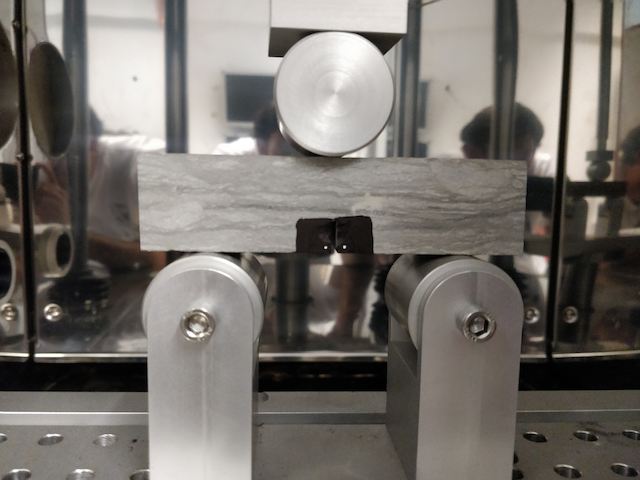
\includegraphics[width=6cm,height=5cm]{figures/Amir_Fracture_Toughness_Setup_a.png}
\subcaption{}
\label{fig:Amir_Fracture_Toughness_Setup_a}
\end{subfigure}
\begin{subfigure}[c]{0.38\textwidth}
\centering
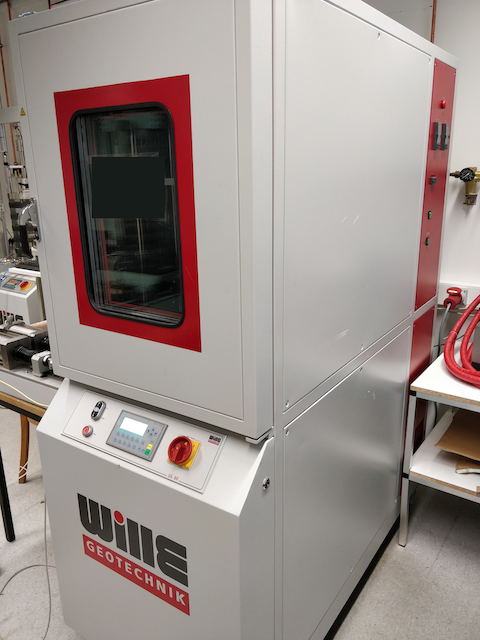
\includegraphics[width=4cm,height=5cm]{figures/Amir_Fracture_Toughness_Setup_b.png}
\subcaption{}
\label{fig:Amir_Fracture_Toughness_Setup_b}
\end{subfigure}
\caption{The required equipment for performing the three-point bending test (a) the loading cell and supports, (b) the climate chamber for controlling temperature and humidity}
\end{figure}

The claystone samples are prepared with the dimension of 140x30x30 $(mm)$ and the notch dimension of 2x10x30 $(mm)$v $(LxWxB)$  (Fig.\ref{fig:Amir_Fracture_Toughness_Sample}). The span length ($S_{flex}$) is 120 $mm$, which is 4 times the size of its width and thickness. The embedded layering is perpendicular to the loading direction. The image processing technique is used to track the reference points, which are predefined prior to the test procedure (Fig. \ref{fig:Amir_Fracture_Toughness_Image_a}). The distance between the points is measured using the optical microscopic image and is considered as an initial reading value (Fig. \ref{fig:Amir_Fracture_Toughness_Image_b}). The method is able to detect the minimum displacement of 2 micrometers, which is possible by taking 4k video with 30fps. The load vs. CMOD response of the Opalinus claystone as well as the numerical simulation outcomes are given in \ref{sec:mex01}. The effects of anisotropy and embedded layering orientation of Opalinus claystones on fracture toughness values are not fully studied. 

\begin{figure}[!ht]
\centering
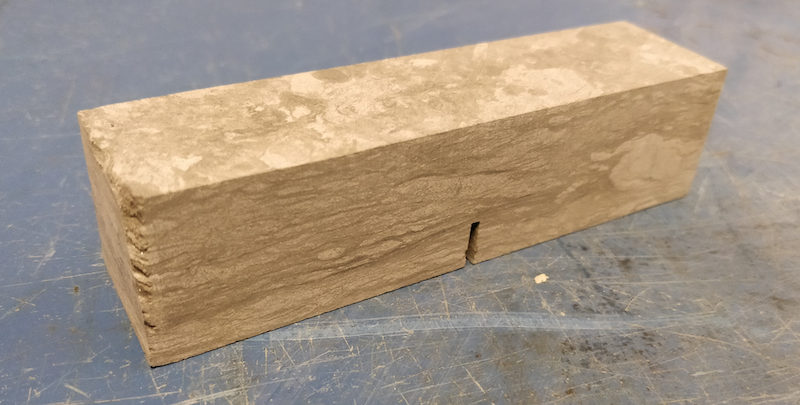
\includegraphics[width=8cm,height=4cm]{figures/Amir_Fracture_Toughness_Sample.png}
\caption{The prepared Opalinus claystone sample with the dimension of 140x30x30 $mm$}
\label{fig:Amir_Fracture_Toughness_Sample}
\end{figure} 

\begin{figure}[!ht]
\centering
\begin{subfigure}[c]{0.48\textwidth}
\centering
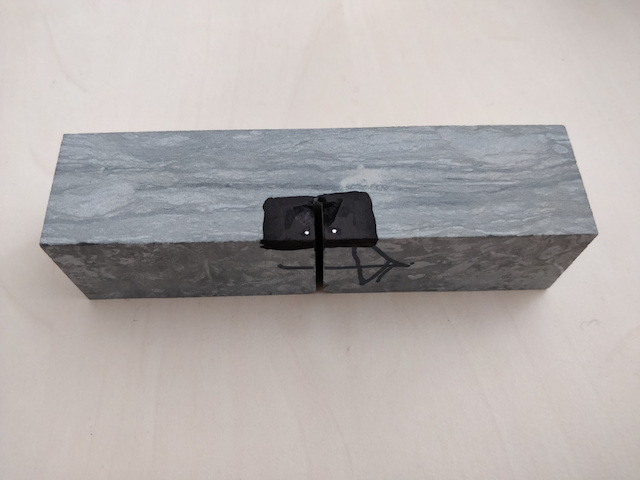
\includegraphics[width=6cm,height=5cm]{figures/Amir_Fracture_Toughness_Image_a.png}
\subcaption{}
\label{fig:Amir_Fracture_Toughness_Image_a}
\end{subfigure}
\hfill
\begin{subfigure}[c]{0.48\textwidth}
\centering
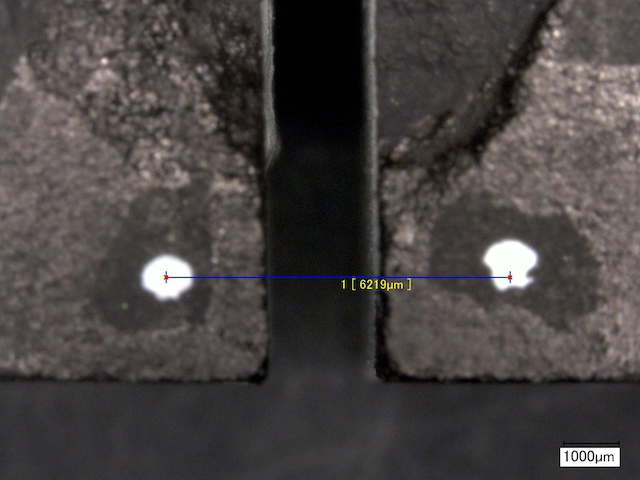
\includegraphics[width=6cm,height=5cm]{figures/Amir_Fracture_Toughness_Image_b.png}
\subcaption{}
\label{fig:Amir_Fracture_Toughness_Image_b}
\end{subfigure}
\caption{The application of image processing technique (a) the predefined reference points for measuring the CMOD, (b) the measured rough distance using optical microscope}
\end{figure}
%---------------------------------------------------------------------------------------------------
\subsection{Brazilian Disk Test on Barrier Rocks}
\label{sec:Brazilian_Disk_Exp}
\Authors{Amir Shoarian Sattari}
%\todo{Please insert authors}

The tensile strength of a brittle or quasi-brittle material, such as rock, is one of the most important material properties, which in comparison to the compression strength, is much weaker. The measurement of direct tensile strength of brittle materials is difficult and time consuming. Therefore, finding the splitting tensile strength ($\sigma_\text{sp}$) is a fast alternative for computing the direct tensile strength. The Brazilian disk test is conducted to determine the splitting tensile strength (Fig. \ref{fig:Amir_Splitting_Theory}). The splitting strength depends on loading rate, diameter and length of the specimen (\ref{eq:Splitting_Strength}). The works of \cite{Perras2014} and \cite{Li2013} provides a full review and a correlation between different rock strength properties.
\index{tensile strength}
\index{compression strength}
\index{Brazilian disk test}

\begin{figure}[!ht]
\centering
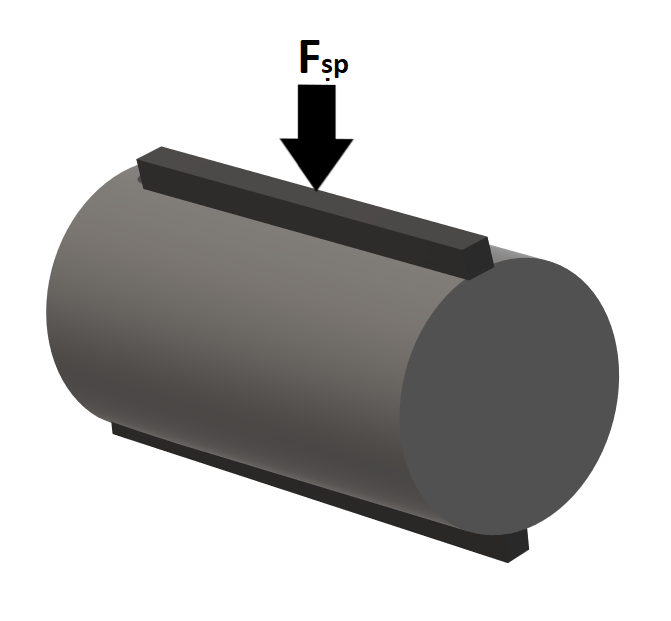
\includegraphics[width=6cm,height=5cm]{figures/Amir_Splitting_Theory.png}
\caption{The Brazilian disk test on a cylindrical sample with diameter and length of $D_\text{cyl}$ and $L_\text{cyl}$, respectively}
\label{fig:Amir_Splitting_Theory}
\end{figure} 

\begin{align}
\label{eq:Splitting_Strength}
\begin{split}
\sigma_\text{sp}=\frac{2f_\text{sp}}{\pi L_\text{cyl}D_\text{cyl}}
\end{split}
\end{align}

In the CAU Kiel laboratory, the splitting strength under THM processes is measured. To do so, a controlled temperature and humidity climate chamber (Fig. \ref{fig:Amir_Fracture_Toughness_Setup_b}) and a loading frame with a displacement transducer are required. Initially, the splitting test under room temperature condition with initial humidity of the sample is conducted. Afterwards, the temperature is raised to 50 and 80 $^{\circ}C$. The relative humidity can be controlled from 0 up to 100. Finally, the splitting strength, splitting Young’ modulus ($E_\text{sp}$) and load-displacement behavior are measured. The cylindrical claystone and saltstone samples are prepared in dimension of 100x200 $mm$ $(DxL)$ (Figure \ref{fig:Amir_Splitting_Sample}) and a strain rate of  0.1 \% is considered to insure a relatively fast loading rate. Fig. \ref{fig:Amir_Splitting_Setup} shows the placement of the sample under loading frame before performing the test.

\begin{figure}[!ht]
\centering
\begin{subfigure}[c]{0.3\textwidth}
\centering
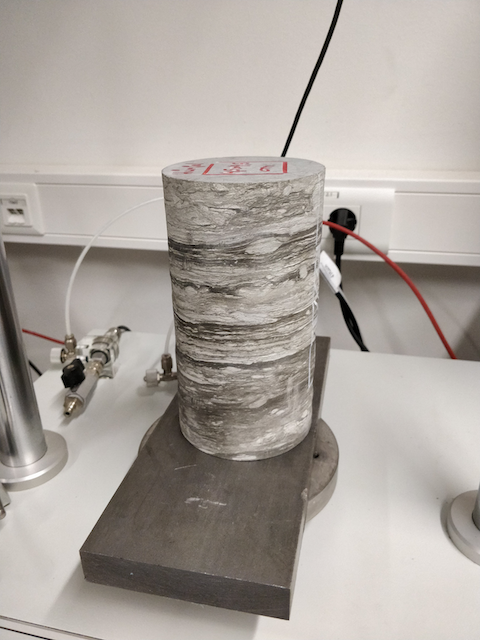
\includegraphics[width=4cm,height=5cm]{figures/Amir_Splitting_Sample.png}
\subcaption{}
\label{fig:Amir_Splitting_Sample}
\end{subfigure}
\hfill
\begin{subfigure}[c]{0.6\textwidth}
\centering
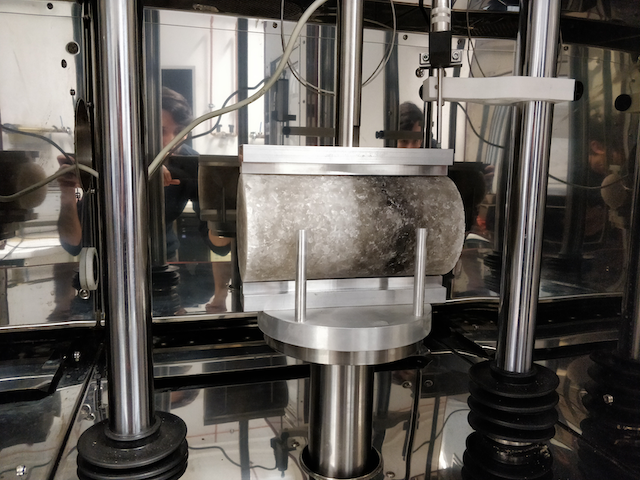
\includegraphics[width=6cm,height=5cm]{figures/Amir_Splitting_Setup.png}
\subcaption{}
\label{fig:Amir_Splitting_Setup}
\end{subfigure}
\caption{The sample preparation and test procedure (a) the claystone sample with a dimension of 100x200 $mm$, (b) the placement of saltstone inside of the climate chamber}
\end{figure}

Initially, the splitting strength of a saltstone samples under room temperature (20), 50 and 80 $^{\circ}C$ are measured. Due to a relatively homogeneous material property of the saltstone, the orientation of the sample will not affect the final outcomes. Figures \ref{fig:Amir_Splitting_Salt_20} and \ref{fig:Amir_Splitting_Salt_Result} depict the failure in 20 $^{\circ}C$ and load vs. displacement for different loading temperatures, respectively. The observed failure pattern for all of the setups is identical. The measured mean splitting strength using equation (\ref{eq:Splitting_Strength}) for 20, 50 and 80 $^{\circ}C$ are 1.65, 1.59 and 1.43 $MPa$, respectively. As a result, the temperature has a slight influence on the splitting strength of saltstone, especially when the temperature is raised up to 50 $^{\circ}C$.

\begin{figure}[!ht]
\centering
\begin{subfigure}[c]{0.35\textwidth}
\centering
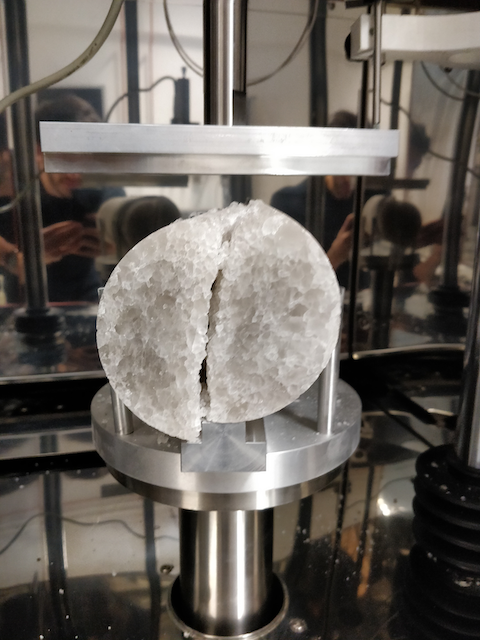
\includegraphics[width=4cm,height=5cm]{figures/Amir_Splitting_Salt_20.png}
\subcaption{}
\label{fig:Amir_Splitting_Salt_20}
\end{subfigure}
\hfill
\begin{subfigure}[c]{0.6\textwidth}
\centering
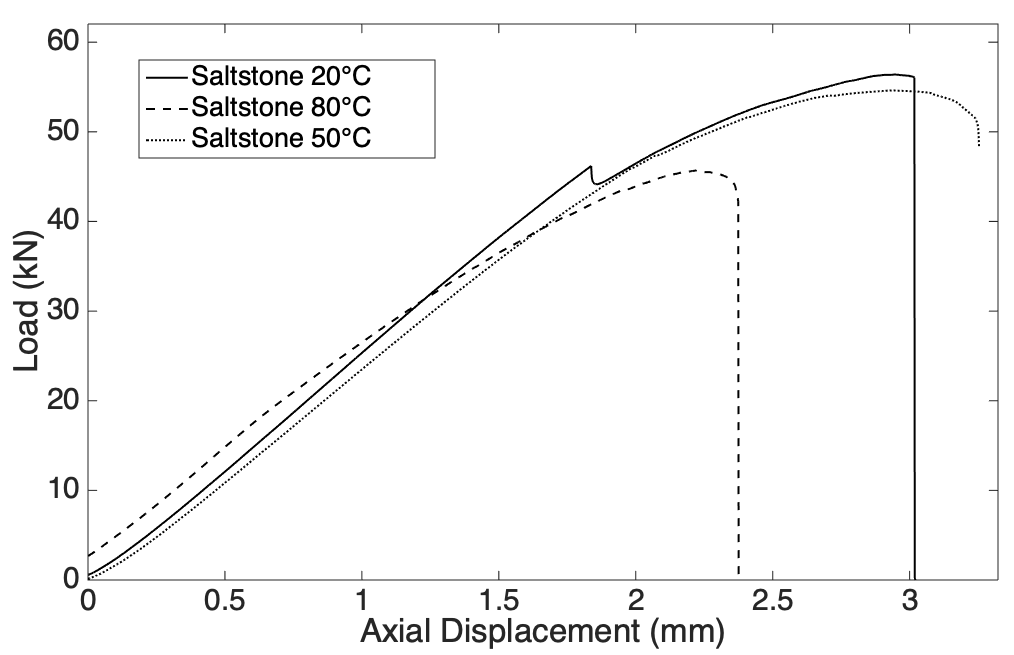
\includegraphics[width=6cm,height=5cm]{figures/Amir_Splitting_Salt_Result.png}
\subcaption{}
\label{fig:Amir_Splitting_Salt_Result}
\end{subfigure}
\caption{The splitting strength of a saltstone under different temperature conditions (a) the fracture path in saltstone in room temperature, (b) the load vs. displacement under different temperature conditions}
\end{figure}

The anisotropy of claystone and embedded layering orientation has a significant influence on material strength. To investigate the strength dependency on layering orientation, a series of tests, where the angle between the loading direction and layering orientation is 0 (parallel), 30, 45, and 90 (perpendicular) degree, is conducted. For 20 $^{\circ}C$, the failure pattern for 0, 45 and 90 degrees are provided in Figures \ref{fig:Amir_Splitting_Clay_0}, \ref{fig:Amir_Splitting_Clay_45} and \ref{fig:Amir_Splitting_Clay_90}. Fig. \ref{fig:Amir_Splitting_Clay_20_Result} depicts the load vs. displacement behavior of claystone with different layering degrees.
\index{anisotropy of claystone}

\begin{figure}[ht!]
\centering
\begin{subfigure}[c]{0.48\textwidth}
\centering
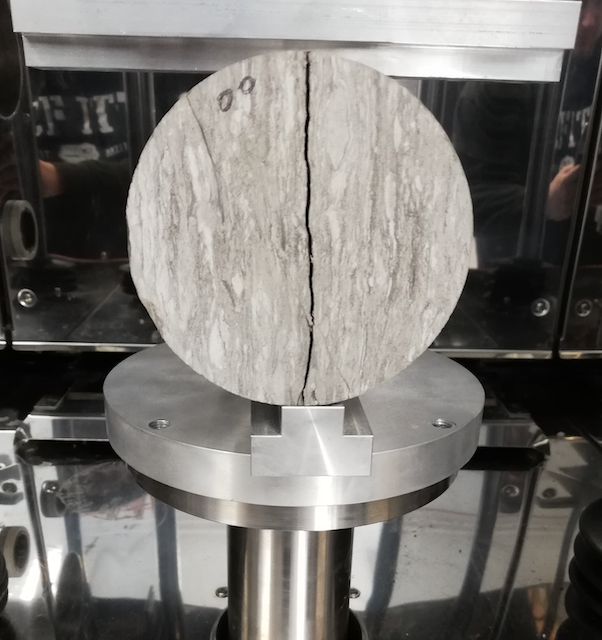
\includegraphics[width=5cm,height=5cm]{figures/Amir_Splitting_Clay_0.png}
\subcaption{}
\label{fig:Amir_Splitting_Clay_0}
\end{subfigure}
\hfill
\begin{subfigure}[c]{0.48\textwidth}
\centering
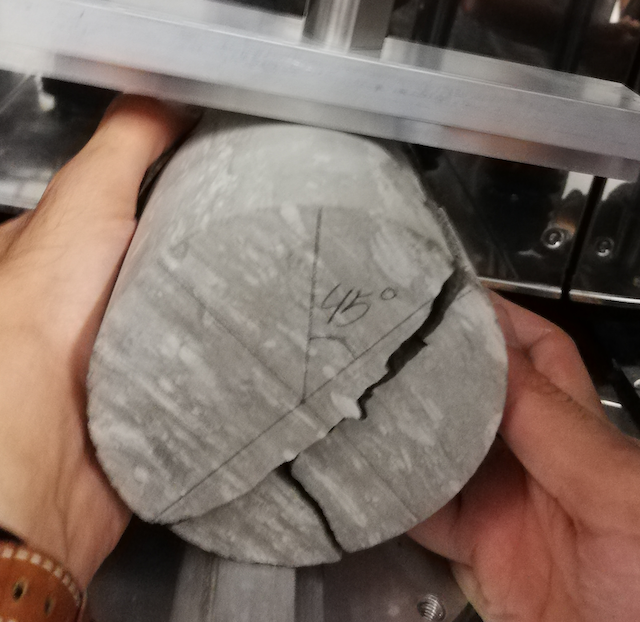
\includegraphics[width=5cm,height=5cm]{figures/Amir_Splitting_Clay_45.png}
\subcaption{}
\label{fig:Amir_Splitting_Clay_45}
\end{subfigure}
\hfill
\begin{subfigure}[c]{0.48\textwidth}
\centering
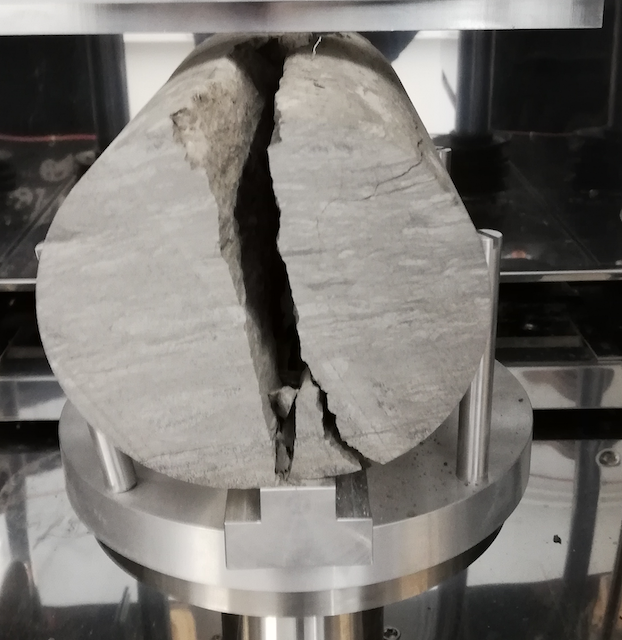
\includegraphics[width=5cm,height=5cm]{figures/Amir_Splitting_Clay_90.png}
\subcaption{}
\label{fig:Amir_Splitting_Clay_90}
\end{subfigure}
\caption{The fracture pattern under different layering orientation (a) 0 degrees, parallel, (b) 45 degrees, and (c) 90 degrees, perpendicular (20 $^{\circ}C$)}
\end{figure}

\begin{figure}[ht!]
\centering
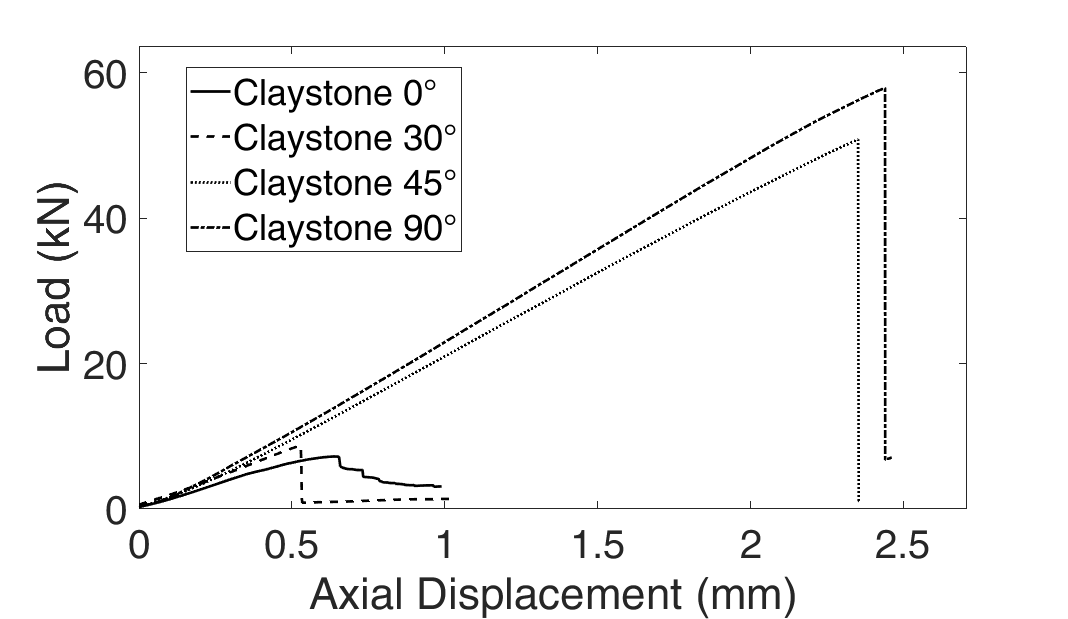
\includegraphics[width=9cm,height=5cm]{figures/Amir_Splitting_Clay_20_Result.png}
\caption{The load vs. displacement under different layering orientation, 20 $^{\circ}C$}
\label{fig:Amir_Splitting_Clay_20_Result}
\end{figure} 

Table \ref{table:Amir_Splitting_Table1} presents the mean outcome of the experimental tests for different orientation angles and temperature. The results depicts that when the loading is perpendicular to the layering orientation, the splitting strength of the claystone is almost 5 times higher than when it is parallel to the layering orientation. The temperature effect on splitting strength is negligible. 

\begin{table}[!ht]
\centering
\begin{center}
\begin{tabular}{ | >{\centering\arraybackslash}X m{8em} | >{\centering\arraybackslash}X m{3em}| >{\centering\arraybackslash}X m{3em} | >{\centering\arraybackslash}X m{3em} | >{\centering\arraybackslash}X m{3em} | >{\centering\arraybackslash}X m{3em} | }
\hline
Test results & 0 $^{\circ}$ & 30 $^{\circ}$ & 45 $^{\circ}$ & 60 $^{\circ}$ & 90 $^{\circ}$ \\
\hline
$\sigma_\text{sp}$ ($MPa$) 20$^{\circ}C$ & 0.47 & 0.68 & 1.13 & 1.45 & 1.92  \\ 
\hline
$\sigma_\text{sp}$ ($MPa$) 80$^{\circ}C$ & 0.52 & 0.64 & 1.02 & 1.25 & 1.86   \\
\hline
\end{tabular}
\end{center}
\caption{The splitting tensile strength of the Opalinus claystone with different temperature and layering orientations}
\label{table:Amir_Splitting_Table1}
\end{table}

%---------------------------------------------------------------------------------------------------
%---------------------------------------------------------------------------------------------------
\subsection{True Triaxial Test on the Cubic Opalinus Claystone Samples}
\label{sec:True_Triaxial_Exp}
\Authors{Amir Shoarian Sattari (CAU)}
%\todo{Please insert authors}

The true triaxial apparatus, where the stresses are controlled along three axes, is used to investigate the three-dimensional strain-strength behavior of soil or rock geomaterial (Figure \ref{fig:Amir_TrueTriaxial_Apparatus}). The true triaxial device in the CAU Kiel laboratory is able to reach a mechanical loading of 600 $MPa$ as well as a thermal loading of up to 600 $^{\circ}C$. The cubic samples are prepared in the side dimension of 43 $mm$ and the edges are slightly curved in order to avoid the stress concentration and failure in the corners (Figure \ref{fig:Amir_TrueTriaxial_Sample}).

\begin{figure}[!ht]
\begin{subfigure}[c]{0.48\textwidth}
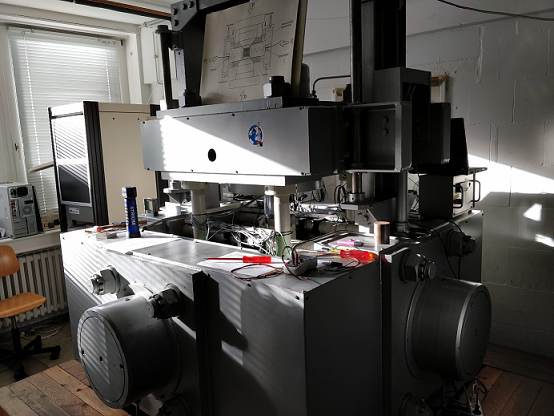
\includegraphics[width=1\textwidth]{figures/Amir_TrueTriaxial_Apparatus.png}
\subcaption{}
\label{fig:Amir_TrueTriaxial_Apparatus}
\end{subfigure}
\hfill
\begin{subfigure}[c]{0.48\textwidth}
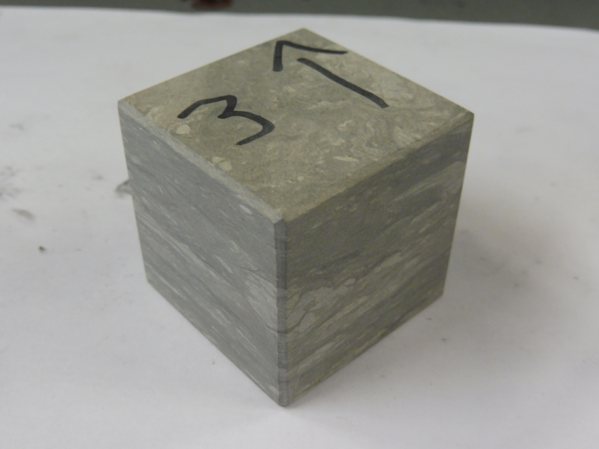
\includegraphics[width=1\textwidth]{figures/Amir_TrueTriaxial_Sample.png}
\subcaption{}
\label{fig:Amir_TrueTriaxial_Sample}
\end{subfigure}
\caption{The (a) true triaxial apparatus in geomechanics laboratory of CAU Kiel, and (b) prepared cubic claystone sample with curved edges}
\end{figure}

The coupled thermo-mechanical loading conditions are considered in order to investigate the materials anisotropic stiffness along three axis, the elastic and plastic deformation under cyclic thermal and mechanical loadings, deviatoric stress field, and material failure. A thermal loading of up to $T_{iso}^{max}=150$ $^{\circ}C$ is considered, which is considered to be higher than the maximum temperature that the claystone samples are subjected to in nuclear waste disposal sites. The maximum isotropic mechanical loading is considered to be $\sigma_{iso}^{max}=100 MPa$, where $max$ and $c$ superscripts represent the maximum and constant values, respectively. The considered boundary conditions are:

\begin{list}{-}{\leftmargin=1em \itemindent=0em \itemsep=0.1em}
  \item Sample MT-01: Mechanical Condition,5 loading cycles, $\sigma_{iso}^{max}=100 MPa$.
  \item Sample MT-02: Coupled Thermo-Mechanical Condition, 4 loading cycles, $T_{iso}^{max}=150$ $^{\circ}C$ and $\sigma_{iso}^{c}=12 MPa$.
  \item Sample MT-03: Coupled Thermo-Mechanical Condition, 4 loading cycles, $T_{iso}^{max}=150$ $^{\circ}C$, and $\sigma_{iso}^{max}=100 MPa$.
  \item Sample MT-04: Coupled Thermo-Mechanical Condition, 4 loading cycles, $\sigma_{dev}^{max}=60 MPa$, $\sigma_{con}^{c}= 20 MPa$ and $T_{iso}^{c}=150$ $^{\circ}C$ .
\end{list}

With the installation of the ultrasonic sensors on the pistons, the apparatus is able to measure the ultrasonic $P$, $S90$ and $S0$ waves along the axis. The anisotropy factor, density ($\rho$), the dynamic Young’s modulus ($E_{Dyn}$), dynamic shear modulus ($G_{Dyn}$), and dynamic Poisson’s ratio ($\nu_{Dyn}$) values can all be calculated according to the analytical relation which already exist in the literature \cite{Motraetal2018} as given in equations (\ref{eq:YoungsModulus_Ultrasonic}) and (\ref{eq:PoissonsRatio_Ultrasonic}). In order to detect and analyse the ultrasonic signals in Opalinus Claystone, the minimum confining mechanical stresses of 12 $MPa$ is required. The test results of MT-01 (Figure \ref{fig:Amir_TrueTriaxial_MT_01_Result}) depicts the increment of the mean $E_{Dyn}$, $G_{Dyn}$ and $\nu_{Dyn}$ values under the isotopic confinement stresses up to 100 $MPa$, which is due to the layering orientation and structure of claystones and eventually improved contact qualities. It is also noted that the rate of the increment after each loading cycle (slope of the line) is decreased and due to the plastic deformations and improved contact qualities, the materials mechanical properties in initial loading condition of 12 $MPa$ are enhanced. 

\begin{figure}[ht!]
\centering
\begin{subfigure}[c]{0.48\textwidth}
\centering
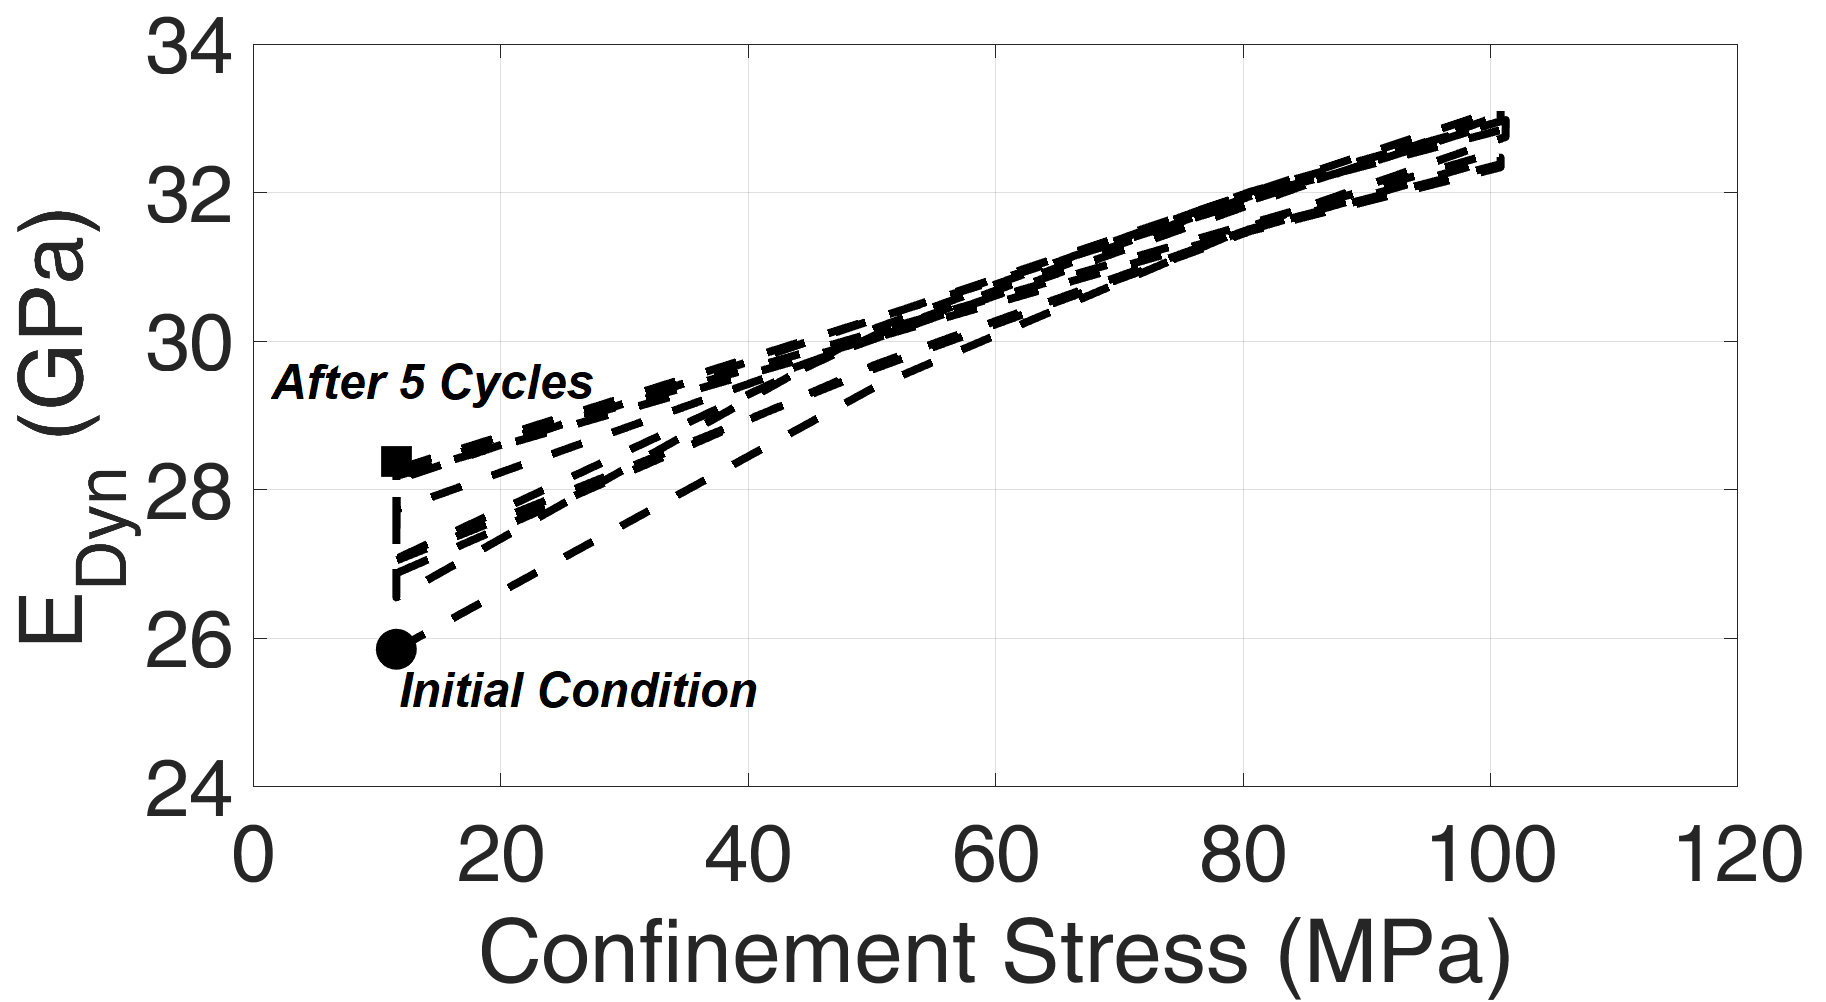
\includegraphics[width=6cm,height=4cm]{figures/Amir_TrueTriaxial_MT_01_Result_E.png}
\subcaption{}
\end{subfigure}
\hfill
\begin{subfigure}[c]{0.48\textwidth}
\centering
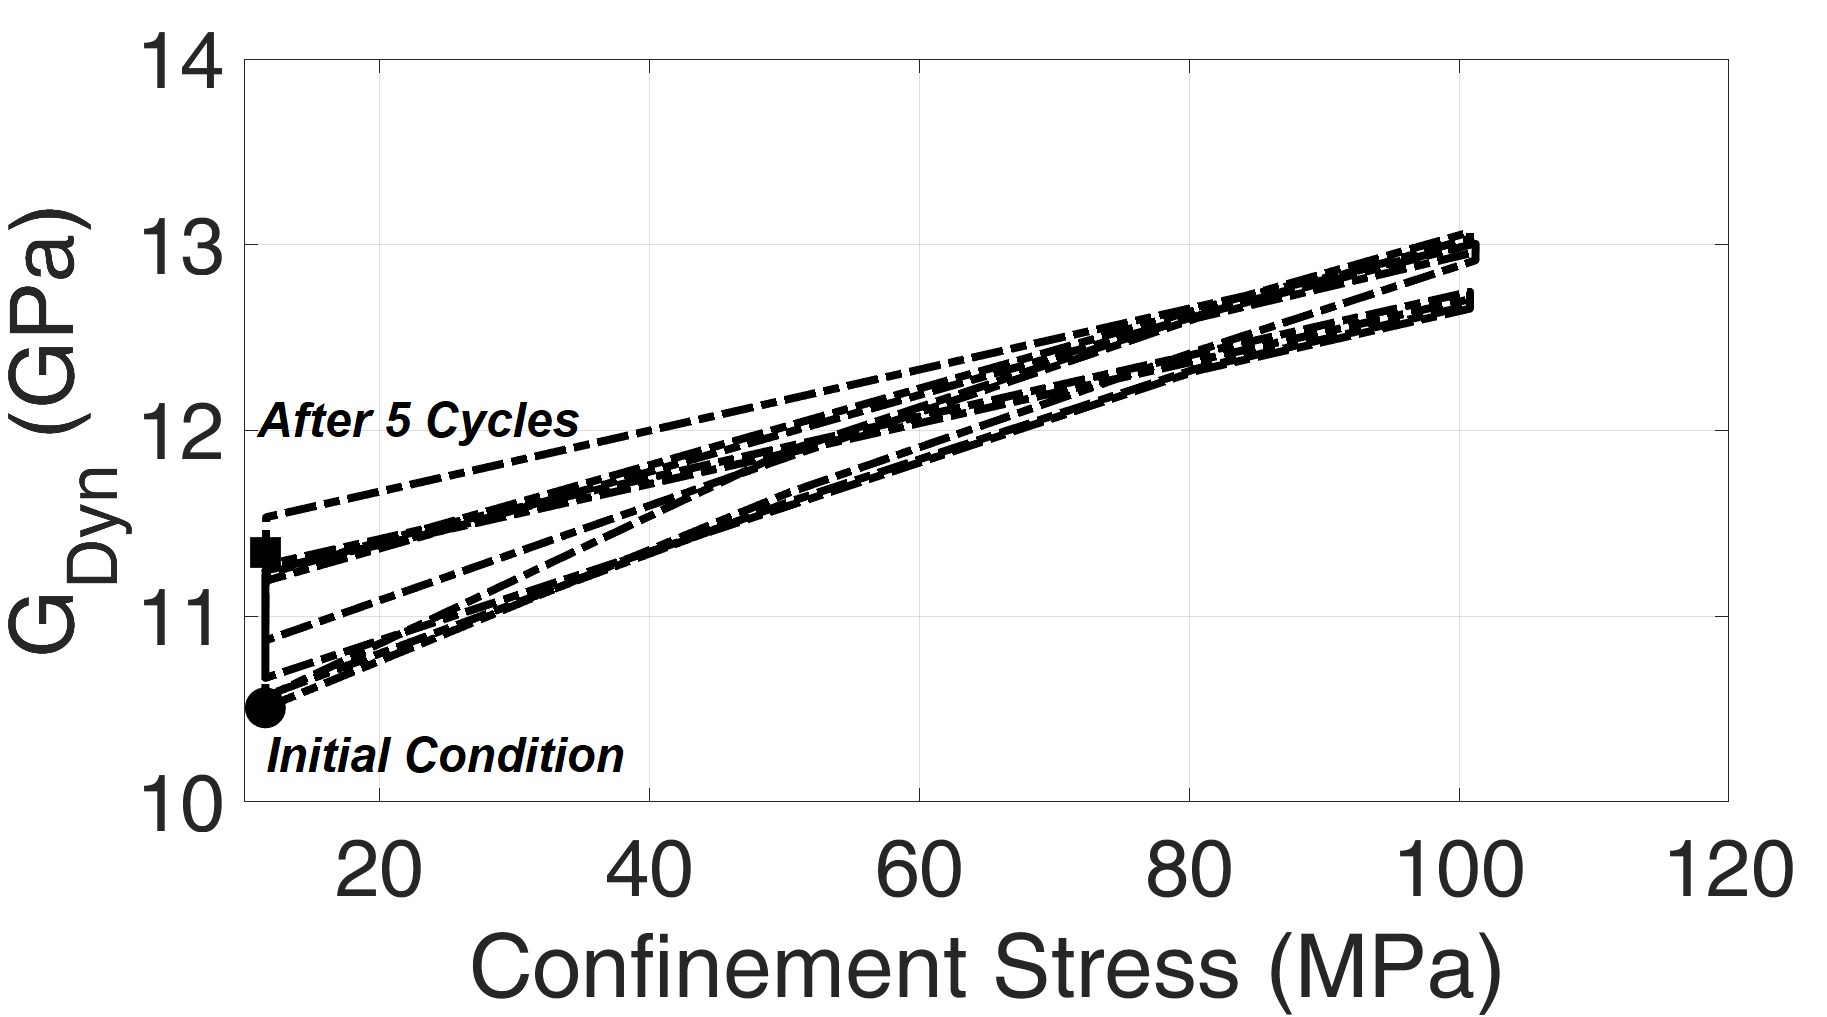
\includegraphics[width=6cm,height=4cm]{figures/Amir_TrueTriaxial_MT_01_Result_G.png}
\subcaption{}
\end{subfigure}
\hfill
\begin{subfigure}[c]{0.48\textwidth}
\centering
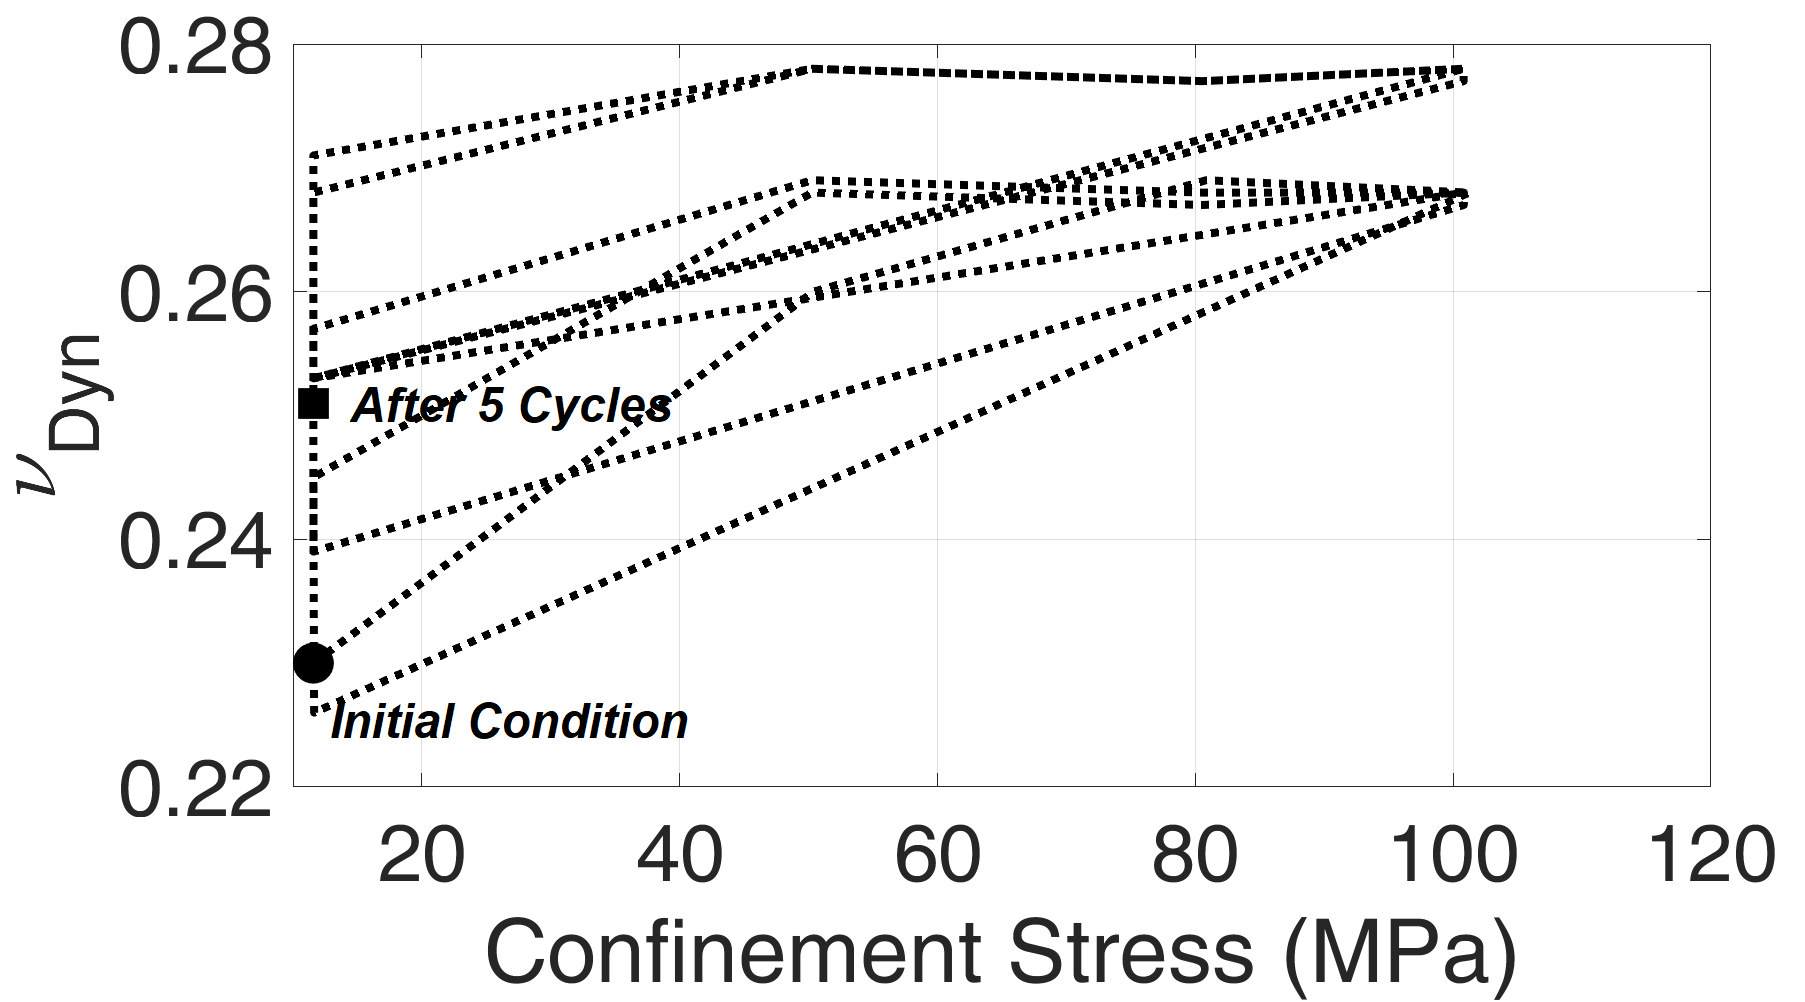
\includegraphics[width=6cm,height=4cm]{figures/Amir_TrueTriaxial_MT_01_Result_Nu.png}
\subcaption{}
\end{subfigure}
\caption{The true triaxial results for the MT-01 sample under 5 loading cycles (a) $E_{Dyn}$ vs. Confinement Stress, (b) $G_{Dyn}$ vs. Confinement Stress, and (c) $\nu_{Dyn}$ vs. Confinement Stress}
\label{fig:Amir_TrueTriaxial_MT_01_Result}
\end{figure}

Figure \ref{fig:Amir_TrueTriaxial_MT_02_Result} shows the deformation vs. time result of MT-02 in the 1st cycle. The thermal plastic deformation after 5 cycles of loading and unloading was negligible and can be neglected. The MT-02 sample is situated in a way that the loading frame in direction of Z is parallel to the layering orientations of claystone. The volumetric thermal expansion coefficient ($\alpha_V$) is calculated based on the measured volumetric strain ($\epsilon_V=\frac{\Delta V}{V}$) and temperature change ($\Delta T$). The effect of temperature on $\alpha_V$ is shown at Figure \ref{fig:Amir_TrueTriaxial_MT_02_Result_1a}. The rate of $\alpha_V$ is decreased after 80 $^{\circ}C$. The anisotropy in linear thermal expansion coefficient along Z, Y and X axis is shown in Figure \ref{fig:Amir_TrueTriaxial_MT_02_Result_1b}. The anisotropy in the measured linear expansion coefficient ($\alpha_{Li}$) is substantially decreased after 80 $^{\circ}C$.

\begin{align}
\label{eq:ThermalExpansion}
\begin{split}
\alpha_V=\frac{\epsilon_V}{\Delta T}=\frac{\Delta V}{V\Delta T}
\end{split}
\end{align}

\begin{figure}[!ht]
\centering
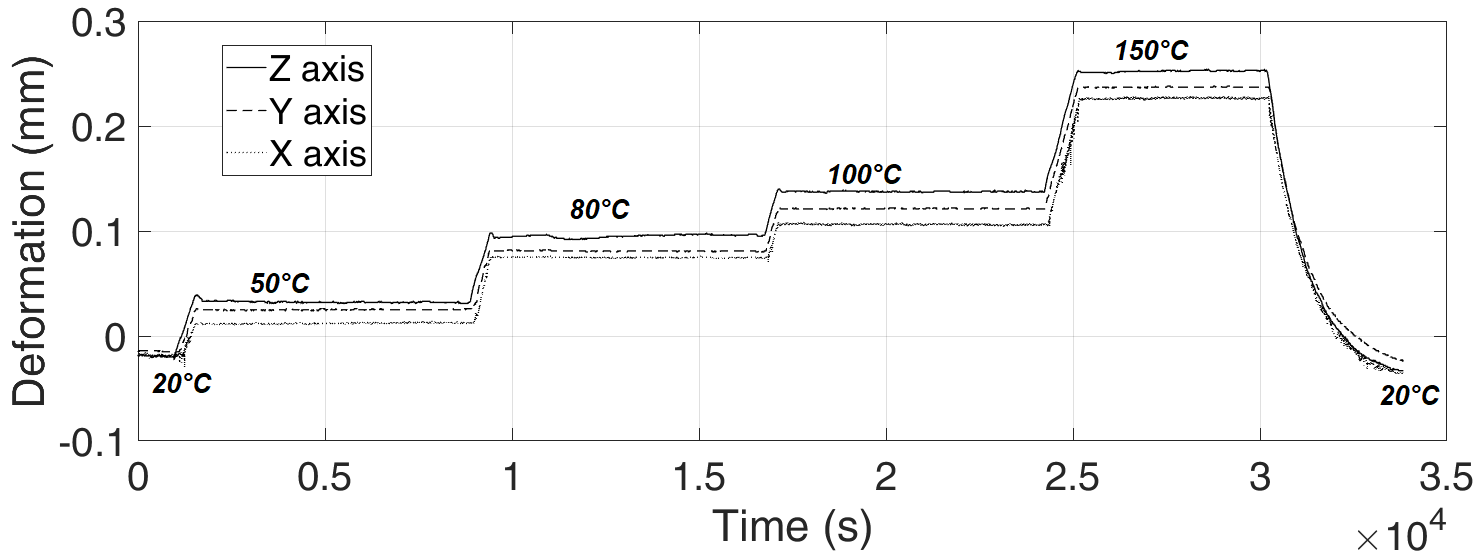
\includegraphics[width=7cm,height=4cm]{figures/Amir_TrueTriaxial_MT_02_Result.png}
\caption{The deformation vs time for sample MT-02}
\label{fig:Amir_TrueTriaxial_MT_02_Result}
\end{figure} 

\begin{figure}[!ht]
\centering
\begin{subfigure}[c]{0.48\textwidth}
\centering
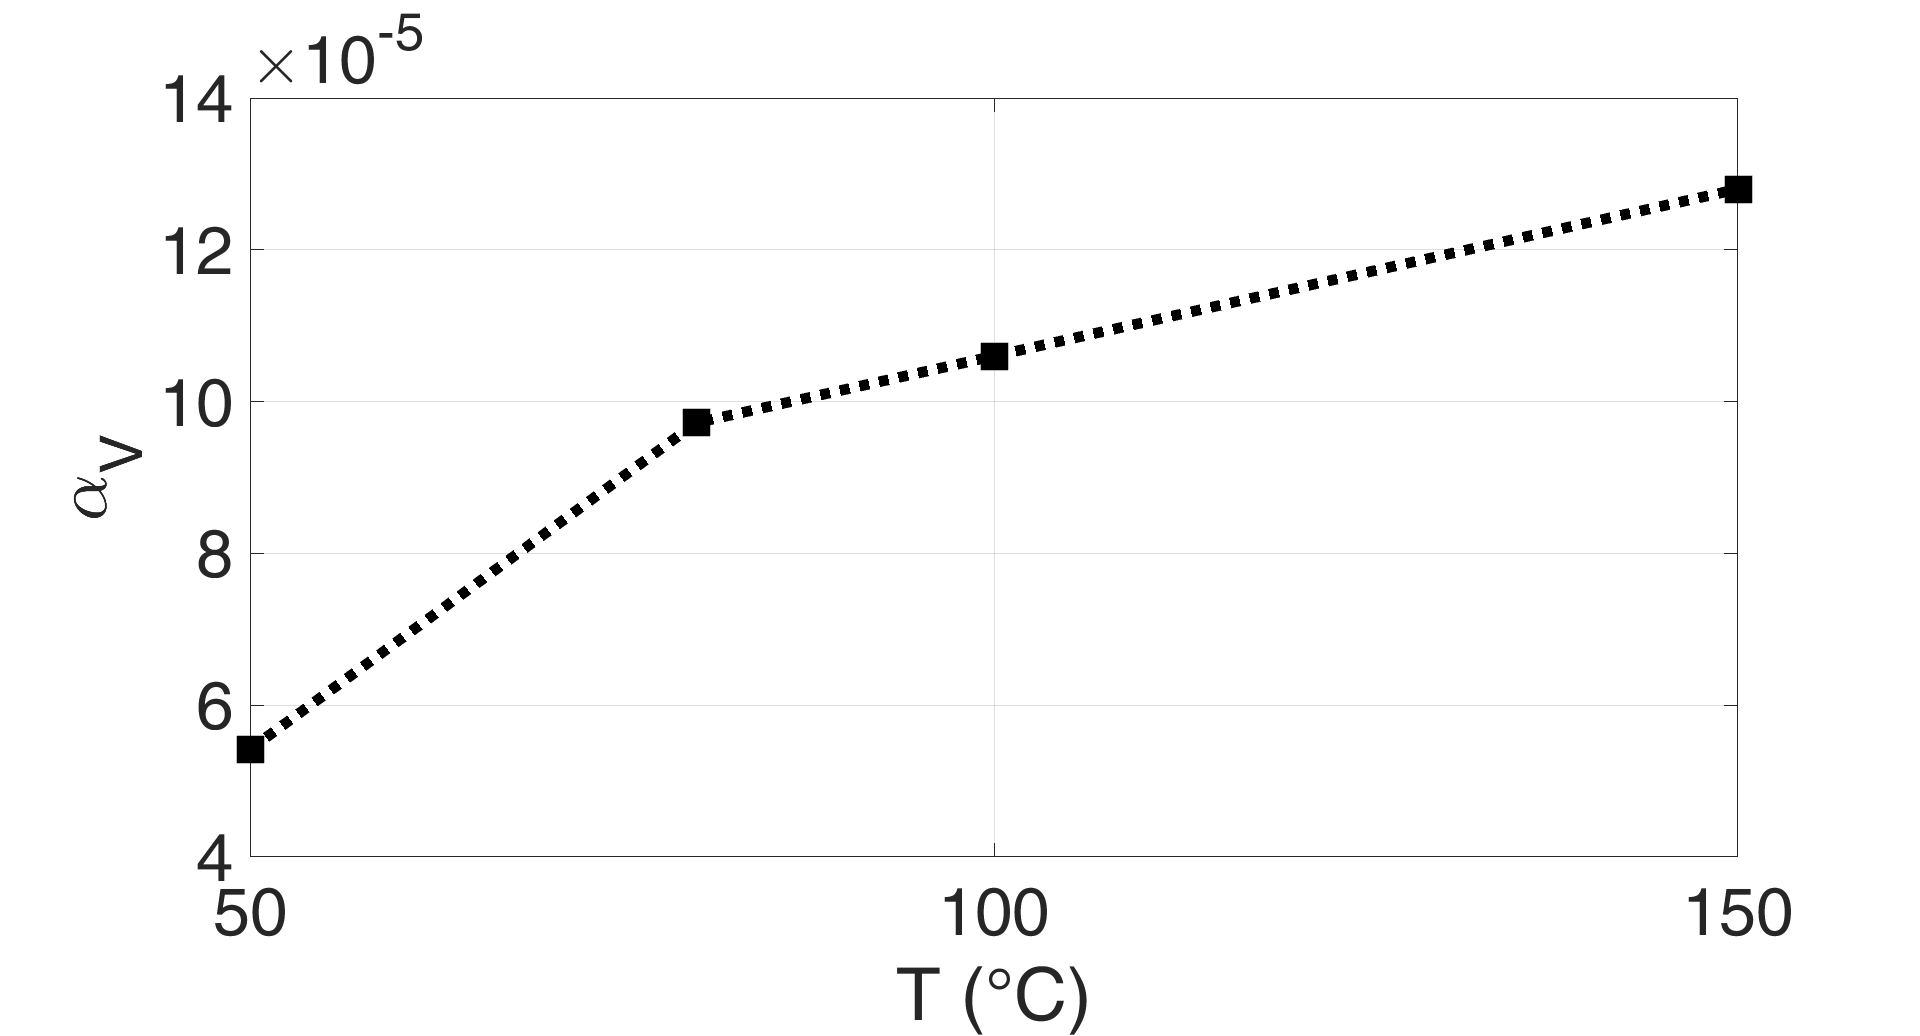
\includegraphics[width=6cm,height=4cm]{figures/Amir_TrueTriaxial_MT_02_Result_1a.png}
\subcaption{}
\label{fig:Amir_TrueTriaxial_MT_02_Result_1a}
\end{subfigure}
\hfill
\begin{subfigure}[c]{0.48\textwidth}
\centering
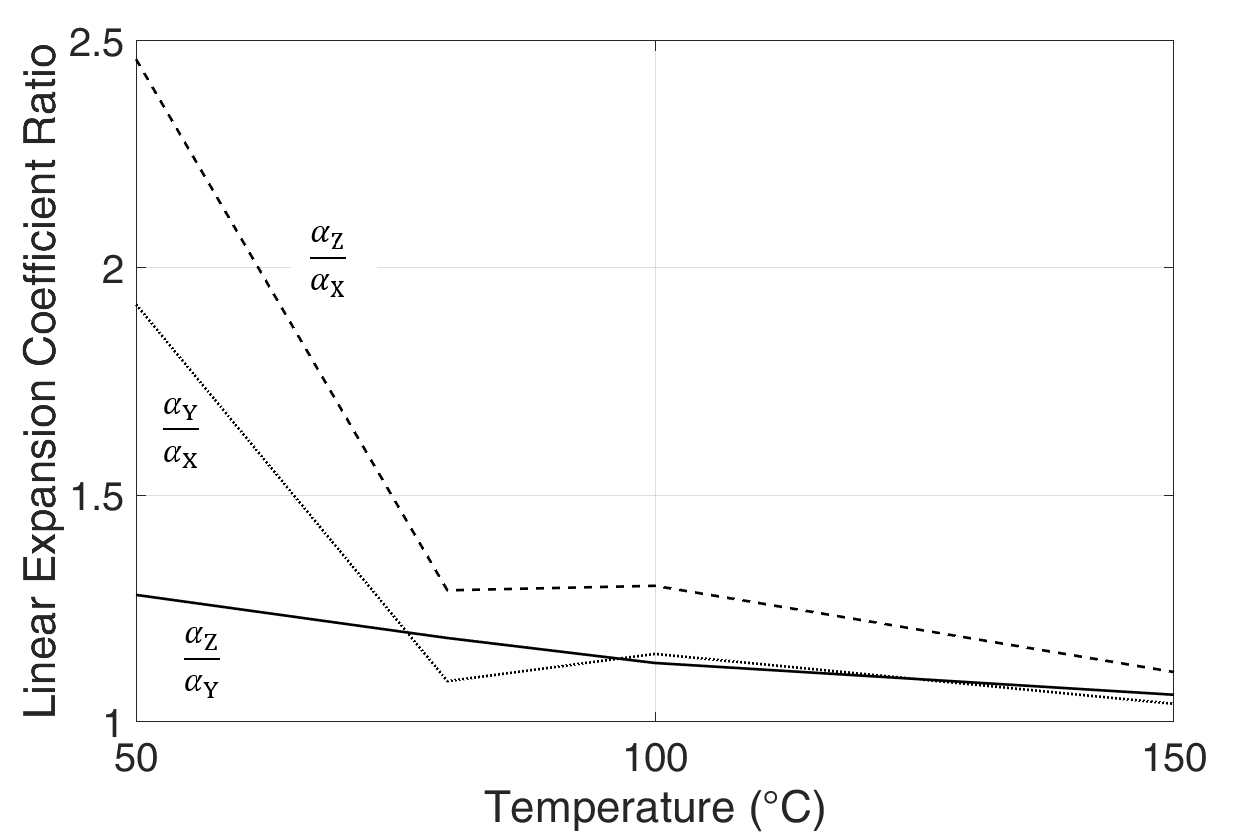
\includegraphics[width=6cm,height=4cm]{figures/Amir_TrueTriaxial_MT_02_Result_1b.png}
\subcaption{}
\label{fig:Amir_TrueTriaxial_MT_02_Result_1b}
\end{subfigure}
\caption{The effect of temperature on (a) $\alpha_V$, and (b) the anisotropy in the linear thermal expansion coefficient ($\alpha_{Li}$)}
\end{figure}

The test results of MT-03 investigates the anisotropy of Opalinus claystone samples. Figure \ref{fig:Amir_TrueTriaxial_MT_03_Result} illustrates the $1^{st}$ cycle loading results of $E_{Dyn}$ and $\nu_{Dyn}$ values in X, Y and Z directions under the isotopic confinement stresses up to 100 $MPa$. The $G_{Dyn}$ has a similar behavior to the $E_{Dyn}$ values. The results indicate a weaker stiffness in Z direction, which is parallel to the layering orientation. The thermal loading upto 150 $^{\circ}C$ results in weaker $E_{Dyn}$ values during the heating process, which is the reason for the fluctuation of the results at the confinement stress of 100 $MPa$. The test results of MT-04 is similar to the MT-02 and the same material response is observed. 

\begin{figure}[ht!]
\centering
\begin{subfigure}[c]{0.48\textwidth}
\centering
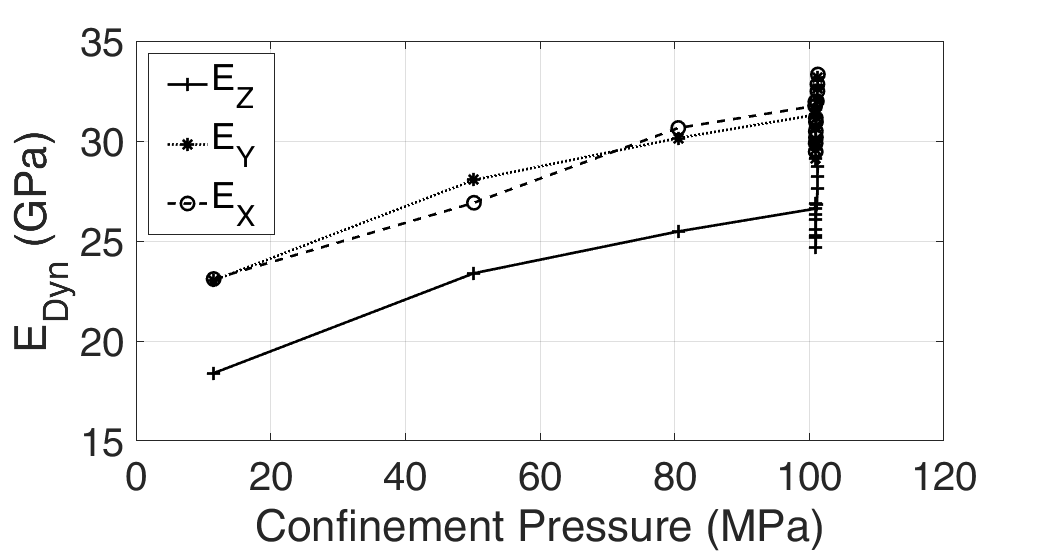
\includegraphics[width=6cm,height=4cm]{figures/Amir_TrueTriaxial_MT_03_Result_E.png}
\subcaption{}
\end{subfigure}
\hfill
\begin{subfigure}[c]{0.48\textwidth}
\centering
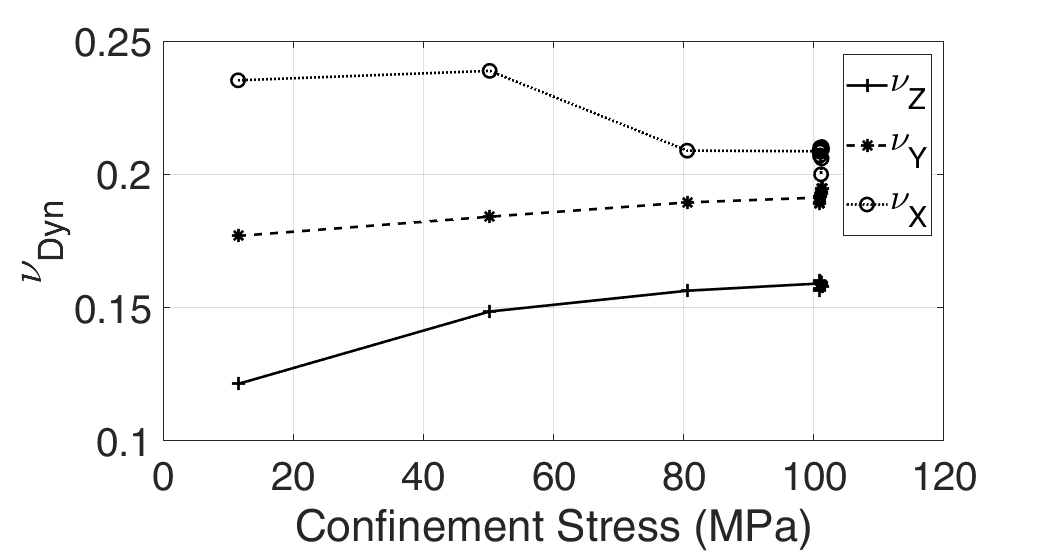
\includegraphics[width=6cm,height=4cm]{figures/Amir_TrueTriaxial_MT_03_Result_Nu.png}
\subcaption{}
\end{subfigure}
\caption{The true triaxial results for the MT-03 sample in the $1^{st}$ cycle (a) $E_{Dyn}$ vs. Confinement Stress, and (b) $\nu_{Dyn}$ vs. Confinement Stress}
\label{fig:Amir_TrueTriaxial_MT_03_Result}
\end{figure}
%---------------------------------------------------------------------------------------------------
\clearpage
%===================================================================================================
\section{Shrinkage and Swelling Laboratory Tests (WP1)}
\label{sec:lab-wp1}
\subsection{The Swelling Characteristic of the Opalinus Claystone}
\Authors{IfG}
\todo[inline]{[IfG](): The description of the experiment procedure}

%---------------------------------------------------------------------------------------------------
%\subsection{Oedometer Test (BGR)}
%---------------------------------------------------------------------------------------------------

\subsection{The Wetting and Drying Paths of the Opalinus Claystone}
\label{sec:Shrinkage_Swelling_Exp}
\Authors{CAU Kiel}
%\todo{Please insert authors}

The shrinkage and swelling of claystone results in micro fracking and higher permeability values, which in nuclear waste disposal sites can lead to contamination of groundwater. Micro fracking also decreases the strength of the material subjected to THM  loading processes. Typically, the swelling pressure and heave of claystone is determined using Oedometer tests \cite{Peronetal2009}, where a constrained or unconstrained sample is subjected to the swelling process (Figure \ref{fig:Amir_Shrinkage_Swelling_Setup}). During the test procedure, the swelling pressure, as well as the heave magnitude, are recorded. It is observed that the swelling pressure in sandy facies of claystone is lower than shaly facies. In contrast to the swelling tests, shrinkage tests are less common and are complicated to perform on rock materials. \cite{Minardietal2016} performed a shrinkage test on claystone with shaly and sandy facies using a desiccator and various salt solutions (Figure  \ref{fig:Amir_Shrinkage_Minardi}). During the test procedure the axial strain values obtained from the strain gauges, as well as sample weight, are measured.

\begin{figure}[!ht]
\begin{subfigure}[c]{0.48\textwidth}
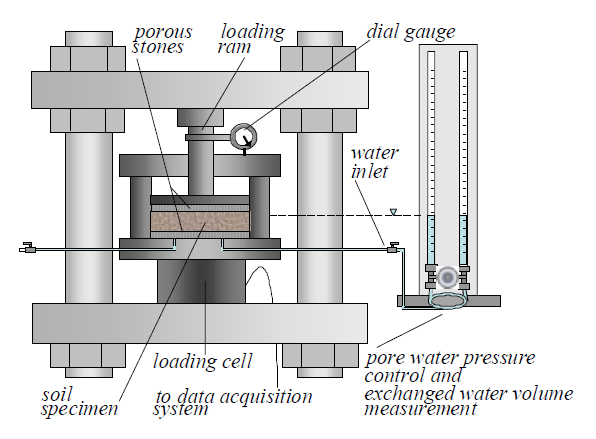
\includegraphics[width=1\textwidth]{figures/Amir_Shrinkage_Swelling_Setup.png}
\subcaption{}
\label{fig:Amir_Shrinkage_Swelling_Setup}
\end{subfigure}
\hfill
\begin{subfigure}[c]{0.48\textwidth}
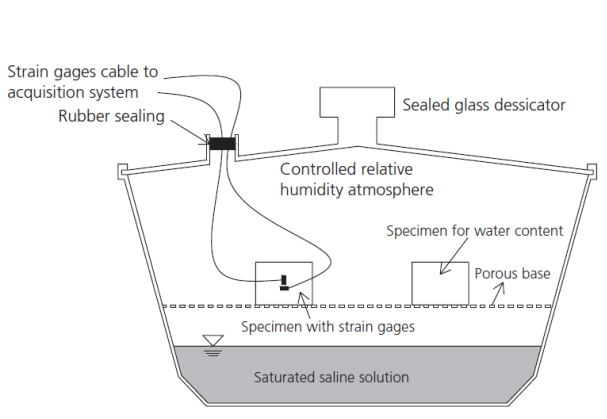
\includegraphics[width=1\textwidth]{figures/Amir_Shrinkage_Minardi.png}
\subcaption{}
\label{fig:Amir_Shrinkage_Minardi}
\end{subfigure}
\caption{The swelling and shrinkage tests on Opalinus claystone (a) the Oedometer test setup for constrained swelling pressure in Opalinus clay samples \cite{Peronetal2009}, and (b) measuring the drying and wetting paths using desiccator \cite{Minardietal2016}}
\end{figure}

Two prepared thin cylindrical sections of sandy Opalinus claystone (Mont-Terri) with a dimension of 100x10 $mm (DxH)$ are used to determine the anisotropy in shrinkage and swelling behavior of claystone. Due to the mineral structure of claystone and its layering orientation, the anisotropy factor has a significant influence on the direction of shrinkage and swelling as well as the micro fracking formation. The initial sample is used to determine the axial strains in parallel and perpendicular directions to the layering orientations. The strain gauge strips (HBM, $LY 10 (mm)$/120 $\Omega$) are glued and attached to the surface of the sample. The second sample is used to measure the weight change in the sample under different salt solutions. The saturated salt solutions are located inside the desiccator and will result in osmotic suction and eventually in the wetting and drying of the samples. The total suction($\psi_{total}$) value can be measured using the Kelvin’s relation, which is derived from ideal gas law:

\begin{equation}
\label{eq:Total_Suction}
\psi_{total} = \frac{RT}{V_{mol}} \ln(\frac{P_{vap}^{cur}}{P_{vap}^{cur=0}})
\end{equation}

where, $(\frac{P_{vap}^{cur}}{P_{vap}^{cur=0}})$ is the relative humidity, $P_{vap}^{cur=0}$ is the vapor pressure when the surface curvature is equal to zero (flat surface), $R$ is the universal gas constant, $T$ is the temperature and $V_{mol}$ is the molecular volume of water. The equilibrium inside the desiccator is reached when the strain gauges value or water content of the samples are constant in two consecutive readings. The results obtained from the drying and wetting paths of the Opalinus claystone are given in \ref{sec:mex06}, where a numerical simulation and comparison to the experimental data are provided. The test procedure is time consuming and after measuring the data for more than 120 days, the applied suction and water content percentages are calculated and plotted. 

%---------------------------------------------------------------------------------------------------
\subsection{In-situ Condition Desiccation Process (Stuttgart or BGR)}
\todo[inline]{[UoS/BGR](): More description please}
Topology, respectively morphology investigations of fractures induced in clay stone throughout drying processes require a number of experimental sequences ranging from the drying process itself to characterization of the induced fractures by X-Ray Computed Tomography. The required samples are prepared and characterized by the University of Kiel with a dimension of radius $r = 5 \, \text{mm}$ and height $h = 50 \, \text{mm}$ to guarantee the realization of scans in Regions of Interests (RoIs) down to a characteristic edge length of $6 \, \text{mm}$ resulting in a resolution of 2 micrometers per voxel.

Two different experimental set-ups are planned; nevertheless the first proposed experimental implementation is preferred over the second.

\subsection{Drying Wet Samples - From Wet to Dry}
\todo[inline]{[UoS](): More description please}
Saturated samples are prepared by the University of Kiel and submerged in a shrink tube in order to minimize the change of the desired state. Once the experiments are performed on the sample the shrink tube is removed and the probe is installed in an uni-axial testing device. The sample is installed in a heat chamber and loaded by an axial force of $f_{ax} = 500 \, \text{N}$/, resulting in an axial stresses of $ \sigma_{ax} = 0.25 \text{MPa}$ (potentially up to $f_{ax} = 5 \, \text{kN}$/$ \sigma_{ax} = 2.5 \text{MPa}$) while axial deformations are measured under controlled temperature conditions. By measuring the sample's weight at characteristic states (twice - beginning and end) the volumetric deformations can be determined and related to the change of saturation. The sample characterization is then completed by XRCT scans to determine the features of the induced fractures. Finally the stiffness degradation is determined by ultrasound experiments measuŕing the P-wave run times at 2, respectively 6 MHz.

\subsection{Wetting dry Samples - From Dry to Wet}
\todo[inline]{[UoS](): More description please}

Since it is extremely time consuming to increase the saturation of the sample this second setting is only an alternative to the introduced set-up in case the first experiment fails. The set-up is comparable to the proposed experiment but performed in a heat-humidity chamber at rel. humidity between 10 - 90 \% and temperatures between $5-90^\circ C$. The applied axial Force would reduce to $f_{ax} = 50 \, \text{N}$.
\clearpage
%---------------------------------------------------------------------------------------------------
\section{Pressure Driven Percolation Laboratory Tests (WP2)}
\label{sec:lab-wp2}
%===================================================================================================
%---------------------------------------------------------------------------------------------------
\subsection{Pressure Driven Percolation}
\Authors{IfG}
%\todo{Please insert authors}

The determination of the permeability, which quantifies the flow behavior of fluids in the pore space of a rock, is based on the Darcy equation:
\index{Darcy equation}

\begin{equation}
q = \frac{kA}{L\eta}\Delta p
\end{equation}

with:
\begin{tabbing}
sym \= description \kill
$q$ : \> flow rate (m$^3$/s) \\
$k$ : \> permeability (m$^2$) \\
$A$ : \> cross sectional area (m$^2$) \\
$L$ : \> length of sample (m) \\
$\eta$ : \> dynamic viscosity (Pa$\cdot$ s) \\
$\Delta p$ : \> pressure difference (Pa)
\end{tabbing}

Thereafter, the flow rate of a fluid through a sample at a given pressure differential is measured by the viscosity of the flowing medium, the geometric factor of the sample, and the permeability (with the dimension of an area). The permeability is given as SI-unit in (m$^2$ or, traditionally, in D (Darcy) (1 D corresponds to about 10$^{-12}$ m$^2$).

The equation above is only valid for incompressible fluids, because only then is the flow rate $q$ constant over the flow path. With sufficient accuracy, this applies to low compressible fluids.
When a gas flows through the pore space of a solid, however, an expansion of the gas takes place along the flow path, so that the flow rate is not constant here. In this case, instead of the flow rate $q$ the mean flow rate $q_m$ is set, for which, for small pressures with sufficient accuracy according to the law of Boyle-Mariotte:
\index{Boyle-Mariotte law}

\begin{equation}
q_m p_m = q_0 p_0
\end{equation}

with:
\begin{tabbing}
sym \= description \kill
$q_m$ : \> mean flow rate \\
$p_m$ : \> mean pressure \\
$q_0$ : \> measured flow rate at $p_0$ \\
$p_0$ : \> pressure at flow rate measurement 
\end{tabbing}

If, for the mean pressure $p_m$, the arithmetic mean of the pressures $p_1$ on the high pressure side and $p_2$ on the low pressure side of the porous solid is used, taking into account that $\Delta p = p_1 - p_2$, the modified Darcy equation for gas flows is as follows:

\begin{equation}
k = \frac{2p_0q_0\eta L}{A(p_1^2-p_2^2)}
\end{equation}

In summary, the determination of the permeability with caustic or gas with knowledge of the viscosity requires in each case an exact measurement of the flow rate after setting (quasi) stationary flow conditions and the pressure gradient.

To carry out permeability tests, the IfG Leipzig uses a servo-hydraulic testing machine with a pressure cell up to pc-max = 1000 bar, which is otherwise used for strength tests with $F_{max}$ = 2500 kN (manufacturer: Schenk / Trebel) (Fig. \ref{fig:ifglabph4}). The tests routinely set hydrostatic pressure conditions ($\sigma_1 = \sigma_2 = \sigma_3$), but it is also possible to implement deviatoric stresses or defined deformations. The axial load or deformation and the jacket pressure are each controlled 
independently via a servo-hydraulic system. 

The desired jacket pressure is generated by a pressure intensifier. From the axial deformation and the measured change in volume of the lateral pressure chamber (piston displacement of the pressure booster), the volume change of the test specimen, referred to here as dilatancy, can be determined at constant jacket pressure.

In hydrostatic loads sintered metal plates are used, which allow over the entire cross-sectional area of the sample a fluid pressurization. The pressure measurement of the measuring fluid is carried out by pressure transducers from Hottinger (accuracy class 0.2), whereby depending on the measuring range a 20 bar or 200 bar encoder is used.

\begin{figure}[!ht]
\centering
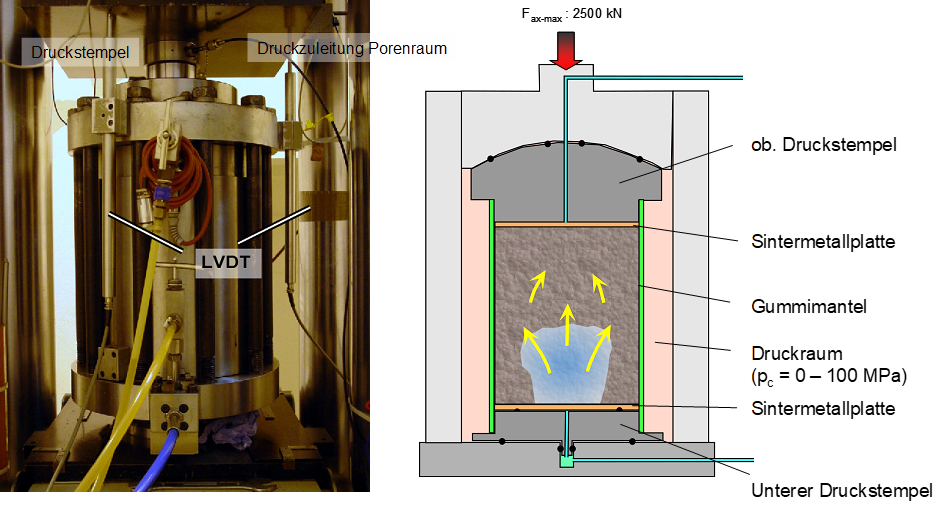
\includegraphics[width=1\textwidth]{./figures/ifg-lab-photo4.png}
\caption{Triaxial IfG pressure cell for flow tests with brine or gas.}
\label{fig:ifglabph4}
\end{figure}

The measuring principle for permeability determination under stationary conditions is based on the measurement of the flow rate $q$, here under atmospheric conditions ($p_0$), in the axial sample direction at a predetermined pressure gradient $\Delta p = p_1 - p_2$ ($p_1$ = inlet pressure, $p_2$ = outlet pressure).

The measuring arrangement used in the triaxial cell has the following advantages over the frequently used Hassler cells, in which a cylindrical sample is firmly clamped between punches and is only subjected to radial pressure.

\begin{list}{-}{\leftmargin=1em \itemindent=0em \itemsep=0em}
\item Determination of sample deformation during hydrostatic and deviatoric pressurization
\item Use of variable sample geometries (stamp sets between 60 and 110 mm diameter are available, height up to 2 x diameter)
\item The height of the gas injection pressure is limited only by the available gas cylinder pressure (routinely max: 200 bar).
\item For higher gas pressures (up to 1000 bar), a Maximator pneumatic pressure booster is used, but this is only used for special measurements.
\end{list}

For the determination of gas permeability two methods are available:
\begin{list}{-}{\leftmargin=1em \itemindent=0em \itemsep=0.1em}
\item 1st: Injection of nitrogen at a defined injection rate within a range of min. 0.1 ml / min to max. 500 ml / min under 
measurement of the injection pressure when stationary conditions are reached with leakage of the fluid against the atmosphere.
\item 2nd: Injecting nitrogen under a defined pre-pressure and measuring the flow rate at the exit side of the sample against the atmosphere.
\end{list}

\begin{figure}[!ht]
\centering
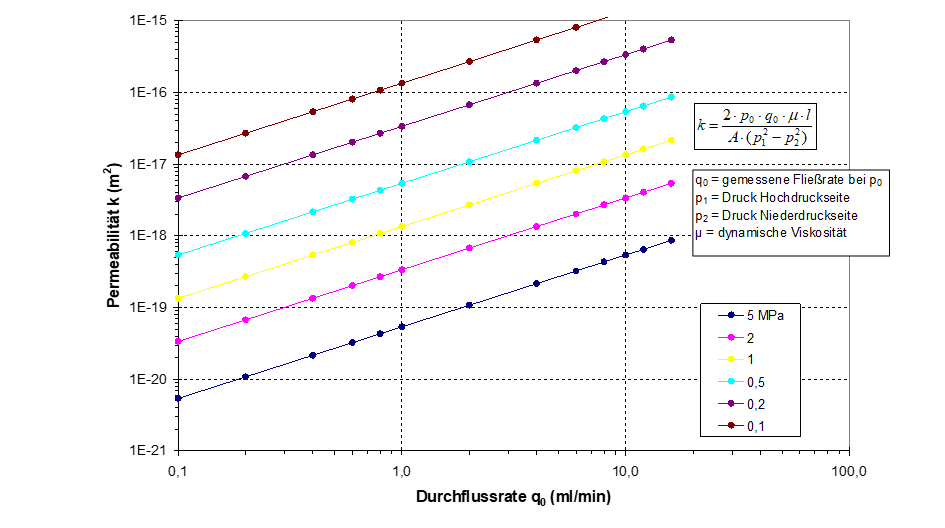
\includegraphics[width=1\textwidth]{./figures/ifg-perme-flowrate.png}
\caption{Variation diagram of permeability vs. flow rate for a sample with l = 220 mm and d = 110 mm at different injection pressures.}
\label{fig:ifgpermeflow}
\end{figure}

The lower limit of the measuring range depends essentially on the pre-pressure or the minimum measurable flow rate, as shown schematically in Fig. \ref{fig:ifgpermeflow}.
%
For gas permeability measurements, EL-FLOW mass flow controllers or flow meters from Bronkhorst are used with the following specifications:

\begin{list}{-}{\leftmargin=1em \itemindent=0em \itemsep=0em}
\item Mass flow controller Type: F-230M: Measuring range: (0) ... 10 ... 500 ml / min N2
\item Form: 200 bar / outlet pressure: 194 bar / temperature: 20$^\circ$C
\item Measuring accuracy: ± 1\% of final value, typ. better 0.5\%
\item Mass flow controller Type: F-230M: Measuring range: (0) ... 0.4 ... 20 ml / min
\end{list}

%---------------------------------------------------------------------------------------------------

\subsection{Fluid Driven Percolation Tests on Cubic Opalinus Claystone samples from Mont-Terri}
\label{sec:Percolation_Claystone_Exp}
\Authors{CAU Kiel}
%\todo{Please insert authors}

The investigation of a fluid transport in claystone due to its anisotropic behavior and its role as a rock barrier in nuclear waste repositories has a great importance. Performing hydraulic fracking under pressurized fluid or storing pressurized fluids leads to the fracking of rock barrier and fluid transport through the hydraulic apertures and cavities. This can lead to pressure and volume drop in the reservoir, decrease the output and efficiency of the designed system and the contamination of ground water. In the geomechanics laboratory of CAU Kiel, the true triaxial apparatus with the maximum mechanical pressure of 600 $MPa$ and thermal loading up to 600 $^{\circ}C$ is used to conduct the fluid driven percolation in claystone samples from Mont-Terri (Figure \ref{fig:Amir_TrueTriaxial_Apparatus}). The syringe pump, with the maximum pressure of 517 $bar$, is used to pressurize the oil fluid. The cubic samples with the side dimension of 43 $mm$ and center hole length and diameter of 20 and 8 $mm$ are prepared (Figure \ref{fig:Amir_Percolation_Adapter}), respectively, and attached to the pump pipes, where the sealing is done with O-rings and epoxy glue (Figure \ref{fig:Amir_Percolation_Setup}). 

\begin{figure}[!ht]
\begin{subfigure}[c]{0.48\textwidth}
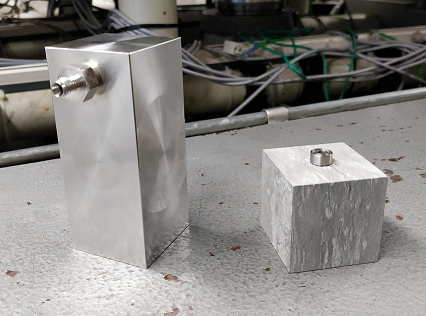
\includegraphics[width=6cm,height=4cm]{figures/Amir_Percolation_Adapter.png}
\subcaption{}
\label{fig:Amir_Percolation_Adapter}
\end{subfigure}
\hfill
\begin{subfigure}[c]{0.48\textwidth}
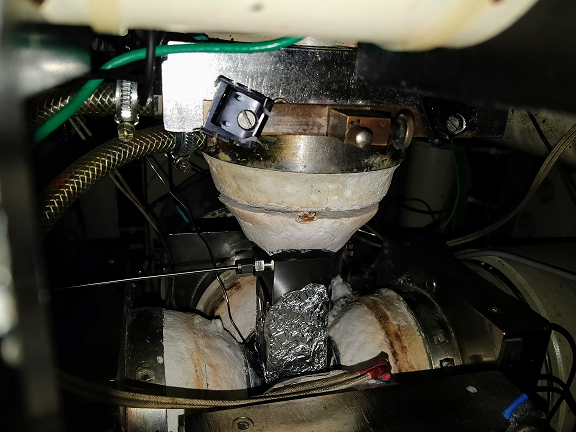
\includegraphics[width=6cm,height=4cm]{figures/Amir_Percolation_Setup.png}
\subcaption{}
\label{fig:Amir_Percolation_Setup}
\end{subfigure}
\caption{The fluid driven percolation test preparation (a) the prepared cubic claystone sample and the adapter¸ and (b) the sample placement inside the true triaxial apparatus}
\end{figure}

Two different stress configurations, as well as fluid injection directions parallel or perpendicular to the layering orientation, are considered to investigate the fracking pattern as well as flow pathways. The fracking tests are carried out under a constant fluid pressure and the peak fluid pressure, where the flow rate increases and any sudden drops in fluid pressure is recorded. In the initial test, a sample with a fluid injection direction perpendicular to the layering orientation of the Opalinus sample is considered (Figure \ref{fig:Amir_Percolation_Orientation1}). The initial stress configuration is 12, 14 and 16 $MPa$ in three different loading directions (Figure \ref{fig:Amir_Percolation_Stress_1}). In order to prevent damaging the sample prior to the hydraulic fracking test, the isotropic stresses of 8 $MPa$ is applied from all pistons and is then gradually increased to the planned stress configuration. The oil pressure is increased gradually up until the point where the borehole pressure drops and an increase in the flow rate can be seen. The test is then aborted immediately in order to avoid causing any damage to the true triaxial apparatus. In the second test setup, a sample with a fluid injection direction parallel to the layering orientation of the Opalinus sample is considered (Figure \ref{fig:Amir_Percolation_Orientation2}). The initial stress configuration is 16, 10 and 8 $MPa$ in three different loading directions (Figure \ref{fig:Amir_Percolation_Stress_2}).

\begin{figure}[!ht]
\begin{subfigure}[c]{0.48\textwidth}
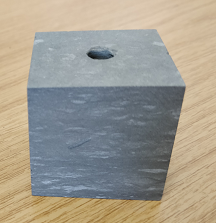
\includegraphics[width=4cm,height=4cm]{figures/Amir_Percolation_Orientation1.png}
\subcaption{}
\label{fig:Amir_Percolation_Orientation1}
\end{subfigure}
\hfill
\begin{subfigure}[c]{0.48\textwidth}
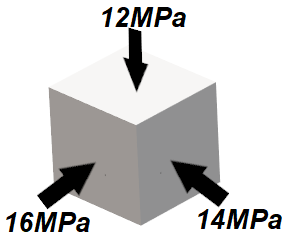
\includegraphics[width=5cm,height=4cm]{figures/Amir_Percolation_Stress_1.png}
\subcaption{}
\label{fig:Amir_Percolation_Stress_1}
\end{subfigure}
\caption{The boundary conditions for the $1^{st}$ stress configuration (a) the orientation of the embedded layers, and (b) the initial stress configuration}
\end{figure}

\begin{figure}[!ht]
\begin{subfigure}[c]{0.48\textwidth}
\includegraphics[width=4cm,height=4cm]{figures/Amir_Percolation_Orientation2.png}
\subcaption{}
\label{fig:Amir_Percolation_Orientation2}
\end{subfigure}
\hfill
\begin{subfigure}[c]{0.48\textwidth}
\includegraphics[width=5cm,height=4cm]{figures/Amir_Percolation_Stress_2.png}
\subcaption{}
\label{fig:Amir_Percolation_Stress_2}
\end{subfigure}
\caption{The boundary conditions for the $2^{nd}$ stress configuration  (a) the orientation of the embedded layers, and (b) the initial stress configuration}
\end{figure}

The results of the percolation tests on the Opalinus claystone samples are given in \ref{sec:mex02}, where a numerical simulation and comparison to the experimental data are provided and the effect of stress distribution, anisotropy and layering orientation on frack paths and fracking pressure are discussed. 

extra comment: change the title of 2.4.1 to be more specific (to show the difference between 2.4.1 and 2.4.2). I suggest: Pressure Driven Percolation Tests on Cylindrical Samples
\clearpage
%---------------------------------------------------------------------------------------------------
\section{Stress Redistribution Laboratory Tests (WP3)}
\label{sec:lab-wp3}
\subsection{Direct Shear Test}
%---------------------------------------------------------------------------------------------------
\Authors{Thomas Fr\"uhwirt, Daniel P\"otschke}

To conduct direct shear tests special equipment is necessary. The direct shear testing device at the rock mechanical laboratory of the TU Freiberg (see Fig. \ref{fig:ExpCNLShearMachine}) is specially developed to ensure the wanted functionality.

\begin{figure}[!ht]
\begin{center}
\includegraphics[width=0.6\textwidth]{./figures/ExpShearMachine.jpg}
\end{center}
\caption{The shear testing device at the rock mechanical laboratory of the TU Freiberg. (From: \cite{Konietzky2012})}
\label{fig:ExpCNLShearMachine}
\end{figure}

Some key features can be found in Table \ref{table:ExpCNLDeviceTechnicalData}. Additionally it is possible to superimpose dynamic forces. In the tests for the GeomInt project this functionality was not used.

\begin{table}[!ht]
\begin{center}
\begin{tabular}{l r r}
Feature & Value & Unit\\
\hline
Max. normal force & 1000 & kN\\
Max. shear displacement & 50 &mm\\
Min. shear velocity & 1e-7 & mm/s\\
Max. shear velocity & 70 & mm/s\\
Max. sample size (rectangular) & 200$\times$400 & mm\\
Max. fluid pressure & 10 & MPa\\
\end{tabular}
\caption{Technical data of the shear testing device. (From: \cite{Konietzky2012})}
\label{table:ExpCNLDeviceTechnicalData}
\end{center}
\end{table}

The sample preparation includes the cutting of the rock block in the cuboid shape. This sample is split into two parts and the rock joints are arranged in a matching position. It is arranged in the shear box, Fig. \ref{fig:ExpCNLSampleInShearBox}.

\begin{figure}[!ht]
\begin{center}
\includegraphics[width=0.6\textwidth]{./figures/ExpCNLSampleInShearBox.jpg}
\end{center}
\caption{Sample in shear box. (From: \cite{Nguyen2014})}
\label{fig:ExpCNLSampleInShearBox}
\end{figure}

The sample is grouted in the shear box to avoid any unwanted movements of it, Fig. \ref{fig:ExpCNLGroutedSample}.

\begin{figure}[!ht]
\begin{center}
\includegraphics[width=0.6\textwidth]{./figures/ExpCNLGroutedSample.jpg}
\end{center}
\caption{Grouted sample before direct shear test. (From: \cite{Nguyen2014})}
\label{fig:ExpCNLGroutedSample}
\end{figure}

The finally equipped shear box is connected to the measuring units, the LVDTs (Linear Variable Differential Transformer), Fig. \ref{fig:ExpCNLLVDT}. The accuracy of this length measurements is in the order of a $\unit[]{\mu m}$.
\index{shear box test}

\begin{figure}[!ht]
\begin{center}
\includegraphics[width=0.6\textwidth]{./figures/ExpCNLLVDT.jpg}
\end{center}
\caption{Measuring equipment: LVDT. (From: \cite{Nguyen2014})}
\label{fig:ExpCNLLVDT}
\end{figure}

The set-up of the experiment is the same for CNL and CNS test. In the CNS test the stiffness which adds an extra load is calculated. This means if a normal displacement of the sample is measured the normal stress will be adapted according to the defined stiffness.
\index{CNL application}
\index{CNS application}

%---------------------------------------------------------------------------------------------------
\subsection{Cyclic Loading Pressure Diffusion}
\Authors{University of Stuttgart}
%\todo{Please insert authors}

In order to study characteristic, time-dependent states of fractures under cycling loading conditions a sample is prepared with a single fracture and borehole before it is installed in a triaxial cell as shown in figure \ref{fig:exp_cyclic_pressure_triax}. The dimension of the sample are chosen to be $r=30 \, \text{mm}$ and height $h=70 \, \text{mm}$. 

\begin{figure}[!ht]
\begin{center}
\includegraphics[width=0.6\textwidth]{./figures/exp_cyclic_pressure_triax.png}
\end{center}
\caption{Set-Up of triaxial cell.}
\label{fig:exp_cyclic_pressure_triax}
\end{figure}

The experiment is performed in three steps. After applying a confining pressure $p_{c}$ the initial state is approached by deformation control while the acting normal forces are measured in a first step. Once a desired normal force is reached the deformation state is held constant and a fluid pressure of $p_{fix}$ is applied. Finally, the fracture is stimulated by a harmonic fluid pressure with a frequency of $0.1 \, \text{Hz}$ and varying amplitudes $p_A$ between $0.5-3 \, \text{MPa}$. Throughout the experiment flow and pressure are measured at the fluid induction point to study the relationship of pressure and flow under non-constant fracture permeabilities triggered by deformations.
\index{cyclic loading test}
%---------------------------------------------------------------------------------------------------
